%%%%%%%%%%%%%%%%%%%%%%%%%%
% A template for PhD and Master's degree theses
%%%%%%%%%%%%%%%%%%%%%%%%%%

\documentclass[12pt,twoside]{book}
\usepackage[margin=1.2in]{geometry}
\usepackage[toc,page]{appendix}
\usepackage{graphicx}
\usepackage[square,numbers]{natbib}
\usepackage{lipsum}
\usepackage{caption}
\usepackage{pdfpages}
\usepackage{url}
\usepackage{wasysym}
\usepackage{xcolor}
\usepackage{amssymb}



\usepackage{amsmath}
\numberwithin{figure}{section}
\numberwithin{table}{section}
\numberwithin{equation}{section}

\usepackage{enumitem}
\usepackage{listings}

\usepackage[acronym,nonumberlist]{glossaries}
\makeglossaries

\newcommand{\myparagraph}[1]{\paragraph{#1}\mbox{}\\[0.3cm]}



\begin{document}

\setcounter{secnumdepth}{3}
\setcounter{tocdepth}{3}

\captionsetup[figure]{margin=1.5cm,font=small,labelfont={bf},name={Figure},labelsep=colon,textfont={it}}
\captionsetup[table]{margin=1.5cm,font=small,labelfont={bf},name={Table},labelsep=colon,textfont={it}}
\SetLipsumDefault{1}

\frontmatter

\begin{titlepage}

% -------------------------------------------------------------------
% You need to edit the details here
% -------------------------------------------------------------------

\begin{center}
{\LARGE Università degli Studi di Bari Aldo Moro}\\[0.25cm]
{\Large Dipartimento di Informatica}\\[1cm]
{\large \emph{Corso di Laurea in\\[1cm]Informatica e Tecnologie per la Produzione del Software}}\\[2.5cm]
\linespread{1.2}\huge {\bfseries Insert Your Title Here}\\[1.5cm]
\linespread{1}

\includegraphics[width=3.5cm]{images/uniba-logo.png}\\[1.5cm]
{\Large\bf Filippo Chinni Carella}\\[1cm]
\large \emph{Supervisor:}\\
Prof. Corrado Mencar\\[1cm] 
\vspace{\fill}
\today
\end{center}

\end{titlepage}

% -------------------------------------------------------------------
% Declaration
% -------------------------------------------------------------------

%\newpage
%\section*{\Large Declaration}

%All sentences or passages quoted in this document from other people's work have been specifically acknowledged by clear cross-referencing to author, work and page(s). Any illustrations that are not the work of the author of this report have been used with the explicit permission of the originator and are specifically acknowledged.  I understand that failure to do this amounts to plagiarism and will be considered grounds for failure.\\[1cm]

%\noindent Name:\\[1mm]
%\rule[1em]{25em}{0.5pt}

%\noindent Signature:\\[1mm]
%\rule[1em]{25em}{0.5pt}

%\noindent Date:\\[1mm]
%\rule[1em]{25em}{0.5pt}

% \includepdf[pages=-]{forms/form.pdf}

\chapter*{\Large \center Acknowledgement}

I am extremely grateful to my supervisor, Prof. Corrado Mencar, for his guidance and support throughout this work.
\\[0.3cm]I would like to thank all members of the Computational Intelligence Laboratory (CILab) for their help and support, especially Prof. Gennaro Vessio and Dr. Pasquale De Marinis for their valuable advice.
\\[0.3cm]I am also grateful to the members of my group projects' team (ABCD), whose help was indispensable for developing the case studies.
\\[0.3cm]I'd like to acknowledge my fellow students, together with whom I have shared funny and memorable moments during the course of my studies.
\\[0.3cm]Finally, I would like to thank my family for their continuous support and encouragement throughout my studies.
\\[0.1cm]
\_\_\_\_\_\_\_\_\_\_\_\_\_\_\_\_\_\_\_\_\_\_\_\_\_\_\_\_\_\_\_\_\_\_\_\_\_\_\_\_\_\_\_\_\_\_\_\_\_\_\_\_\_\_\_\_\_\_\_\_\_\_\_\_\_\_\_\_\_\_\_\_\_\_\_\_\_\_\_\_\_\_\_\_\_\_\_\_\_\_\_\_\_\_\_\_\_\_\_\_\_\_\_\_
\\[0.3cm]
Sono estremamente grato al mio relatore, il Prof. Corrado Mencar, per la sua guida e il suo sostegno durante la stesura di questa tesi.
\\[0.3cm]Vorrei ringraziare tutti i membri del Computational Intelligence Laboratory (CILab) per il loro aiuto e supporto, in particolare il Prof. Gennaro Vessio e il Dott. Pasquale De Marinis per i loro preziosi consigli.
\\[0.3cm]Sono grato anche ai membri del mio team per i lavori di gruppo (ABCD), il cui aiuto è stato indispensabile per lo sviluppo degli casi di studio.
\\[0.3cm]Vorrei riconoscere i miei compagni di corso, con i quali ho condiviso momenti divertenti e memorabili durante il percorso di studi.
\\[0.3cm]Infine, vorrei ringraziare la mia famiglia per il continuo sostegno e incoraggiamento durante i miei studi.

% -------------------------------------------------------------------
% Abstract
% -------------------------------------------------------------------

\chapter*{\Large \center Abstract}

An \emph{abstract} is a summary of a research article, thesis, review, conference proceeding, or any in-depth analysis of a particular subject or discipline. It is often used to help the reader quickly ascertain the article's purpose. Therefore, an abstract should be self-contained and understandable on its own. When used, an abstract always appears at the beginning of a manuscript, acting as the entry point for any academic paper or patent application. Abstracting and indexing services for various academic disciplines are aimed at compiling a body of literature for that particular subject.

% -------------------------------------------------------------------
% Contents, list of figures, list of tables
% -------------------------------------------------------------------

\tableofcontents
\listoffigures
\listoftables

\glsaddall
\printglossary[type=\acronymtype,title=List of Abbreviations]
\printglossary[title=List of Symbols]

% -------------------------------------------------------------------
% Main sections (as required)
% -------------------------------------------------------------------

\mainmatter

%Acronyms and Symbols Lists

\newacronym{ai}{AI}{- Artificial Intelligence}
\newacronym{ml}{ML}{- Machine Learning}
\newacronym{dl}{DL}{- Deep Learning}
\newacronym{nn}{NN}{- Neural Network}
\newacronym{dnn}{DNN}{- Deep Neural Network}
\newacronym{hp}{HP}{- Hyperparameter}
\newacronym{hpo}{HPO}{- Hyperparameter Optimization}
\newacronym{svm}{SVM}{- Support Vector Machine}
\newacronym{bo}{BO}{- Bayesian Optimization}
\newacronym{sgd}{SGD}{- Stochastic Gradient Descent}
\newacronym{pbt}{PBT}{- Population Based Training}
\newacronym{sha}{SHA}{- Successive Halving Algorithm}
\newacronym{asha}{ASHA}{- Asynchronous Successive Halving Algorithm}
\newacronym{bohb}{BOHB}{- Bayesian Optimization and Hyperband}
\newacronym{tpe}{TPE}{- Tree-structured Parzen Estimator}
\newacronym{mab}{MAB}{- Multi-Armed Bandit}
\newacronym{cv}{CV}{- Cross-Validation}
\newacronym{ncv}{NCV}{- Nested Cross-Validation}
\newacronym{cpu}{CPU}{- Central Processing Unit}
\newacronym{gpu}{GPU}{- Graphics Processing Unit}
\newacronym{oo}{OO}{- Object-Oriented}
\newacronym{cma-es}{CMA-ES}{- Covariance Matrix Adaptation Evolution Strategy}
\newacronym{nsgaii}{NSGAII}{- Non-dominated Sorting Genetic Algorithm II}
\newacronym{qmc}{QMC}{- Quasi-Monte Carlo}
\newacronym{psot}{PSO}{- Particle Swarm Optimization}
\newacronym{ga-pso}{GA-PSO}{- Hybrid of Genetic Algorithm and Particle Swarm Optimization}
\newacronym{epso}{EPSO}{- Hybrid of Evolutionary Programming and Particle Swarm Optimization}
\newacronym{apso}{APSO}{- Adaptive Particle Swarm Optimization}
\newacronym{mopso}{MOPSO}{- Multi-Objective Particle Swarm Optimization}
\newacronym{dpso}{DPSO}{- Discrete Particle Swarm Optimization}
\newacronym{mlp}{MLP}{- Multi-Layer Perceptron}
\newacronym{ram}{RAM}{- Random Access Memory}
\newacronym{ssd}{SSD}{- Solid State Drive}
\newacronym{mit}{MiT}{- Mix Transformer}
\newacronym{cnn}{CNN}{- Convolutional Neural Network}

% \newglossaryentry{chi}{
%   name={$\textbf{$\chi$}$},
%   description={ - Space of all possible Hyperparameters Configurations}
% }
% \newglossaryentry{X-bold}{
%   name={$\textbf{X}$},
%   description={ - Search Space}
% }
% \newglossaryentry{X}
% {
%   name={$X$},
%   description={ - Hyperparameter Configuration (or Candidate Solution, or Trial)}
% }
% \newglossaryentry{f}
% {
%   name={$f$},
%   description={ - Objective Function}
% }




% Chapter 1

\chapter{Introduction}

In Machine Learning, the process of training a model involves the optimization of a set of parameters, called Hyperparameters, which are not learned during the training process. The optimization of these hyperparameters is a crucial step in the development of a machine learning model, as it can significantly affect the performance of the model. The process of finding the best hyperparameters for a model is called Hyperparameter Optimization (HPO).
\\[0.3cm]At the current state of research, HPO is a flourishing field, with many different techniques available, ranging from simple traditional manual tuning to more advanced automated optimization algorithms.

\section{Aims and Objectives}

The aim of this thesis is to explore the field of HPO, by testing and comparing different optimization algorithms.
The objectives of the thesis are:
\begin{itemize}[itemsep=0.1cm]
	\item To establish the importance of HPO in Machine Learning and its impact on the training process of a model;
	\item To evaluate the effectiveness of different HPO algorithms, using an existing library for HPO;
	\item To adapt an existing optimization algorithm to make it suitable for HPO, and test its effectiveness; in particular, the algorithm to be adapted is the Particle Swarm Optimization (PSO);
	\item To integrate the adapted algorithm into the existing library for HPO, and test it on different datasets and models;
	\item To test the effectiveness of the HPO algorithms on a more complex dataset, testing the limits and advantages of HPO in a more challenging context. Specifically on a real world problem, in the field of Drone Vision for agriculture.
\end{itemize}
In order to achieve these objectives, a series of experiments will be conducted, where different techniques will be chosen (or developed), analysed and compared. The experiments will be performed mainly on simpler datasets and models to make the process more manageable and to focus attention on the optimization algorithms themselves rather than on specific problems.
\\[0.3cm]Subsequently, with regard to the Drone Vision problem, the experiment will be conducted on a more complex dataset and model. The reason Drone Vision is sensitive to the optimization of hyperparameters is that the functioning of a Machine Learning model, especially Neural Networks which are the most used models in Drone Vision, is highly energetically and computationally expensive. Usually, drones have limited computational resources, therefore, they can hardly afford to run a complex model to perform tasks such as Semantic Segmentation. The proposed methodology aims to perform a weighted Hyperparameter Optimization, where the complexity of the model is penalized, so as to find the best trade-off between performance and computational cost. 
\\[0.3cm]One optimization technique that will get particular attention is the Particle Swarm Optimization (PSO), which is a population-based optimization algorithm inspired by the social behavior of flocks of birds. The algorithm will be adapted to make it suitable for HPO; and then tested, evaluated, and compared. PSO is currently one of the most popular optimization algorithms, therefore, it is interesting to observe its performance in the context of HPO, given its efficacy in searching optimal solutions in high-dimensional spaces. 

\section{Overview of the Thesis}

The rest of the thesis is structured as follows:
\begin{itemize}[itemsep=0.1cm]
    \item \textbf{Chapter 2} provides an overview of the background knowledge about the topic of Hyperparameter Optimization, presenting the state of the art.
    \item \textbf{Chapter 3} describes the methodology used in the experiments, including the models and the algorithms.
    \item \textbf{Chapter 4} presents the results of the experiments, and discusses them.
    \item \textbf{Chapter 5} concludes the thesis, summarizing the results and suggesting future work.
\end{itemize}

\chapter{Background}

According to seminal research by \cite{krizhevsky2012imagenet}, lorem ipsum dolor sit amet. However, this result was already known in the 1990s \cite{lecun1998gradient}. 

\section{Structure and Layout}

Reports written for scientific works, such as degree theses, should feature a specific structure and layout according to well-established standards, which also apply to professional publications of any kind.

In particular, degree theses should have the following contents:
\begin{itemize}
	\item Title page;
	\item Abstract;
	\item Table of contents;
	\item List of symbols (optional);
	\item List of abbreviations (optional);
	\item List of figures (optional);
	\item List of tables (optional);
	\item Text of the thesis, roughly structured as:
	\begin{itemize}
		\item Introduction;
		\item Body;
		\item Conclusion;
	\end{itemize}
	\item Bibliography;
	\item Appendix (optional).
\end{itemize}

An essential aspect is the effective transfer of written information to an educated reader who is not directly familiar with the problem. This includes:
\begin{itemize}
  \item A clear presentation of the evolution of thoughts from the level of knowledge at the beginning of the work to the developed solution;
  \item A good structure and a logical arrangement;
  \item An understandable, short, and exact formulation without deviating from the topic.
\end{itemize}

The level of knowledge is given by the results of preliminary studies and previous publications. Proposals for the problem's solution must be discussed, and the chosen approach has to be justified. Fundamental analysis that does not lead to success must be added with an explanation. The structure and order of the text are based on objective criteria, not on the temporal sequence of development. Subheadings should be well chosen. Frequent hints about the path followed place the sections in context.

The description of the studies and experiments must be detailed enough to allow for replication by others. The results must be reproducible. All tools, such as literature, formulas, programs, or measurement methods, must be indicated. The results or solutions adopted should be explained only to the extent necessary for understanding, with reference to the source but without derivation.

Often, measured and calculated results and functional correlations can be displayed more clearly and understandably with figures or tables than with long descriptions. It is assumed that extensive mathematical derivations or proofs are listed in one or more appendices, as well as collections of figures or tables that break the context of a text passage. The text must include references to all parts of the thesis (figures, tables, literature, attachments).

\subsection{Structure}

\subsubsection{Title Page}

The layout of the title page is given by a template, according to the title page of this guide.

\subsubsection{Table of Contents}

The table of contents consists of the numbered headings of the sections and the corresponding first page numbers. Appendices must also be listed. Page numbering should start with the table of contents as page 1.

Attention should be paid to the consistent capitalization of the headings in the table of contents. Unclear and uncommon abbreviations should be avoided in the headings.

\subsubsection{List of Symbols}

A list of symbols should be provided if the thesis contains many formulas. All symbols used must be arranged alphabetically and described briefly.

\subsubsection{List of Acronyms}

A list of acronyms should be provided if the thesis contains many acronyms, especially within graphics and diagrams. In this list, only uncommon acronyms should be given in alphabetical order and should be briefly described.

\subsubsection{Bibliography}

All sources of information used must be cited in the thesis and listed in the bibliography. In brackets are the reference numbers of the citations. The order of numbering of the cited sources must be that of the first appearance of the citations in the text. When referring to multiple sources, consideration of standardization and uniformity of symbols and abbreviations is required. If necessary, the symbols and abbreviations of the cited sources should be adapted to match the entries in the list of symbols and abbreviations in the thesis. The reference to sources from the Internet is allowed only in special cases, given the vicissitude and transience of these sources. Verify the accuracy of all references, even if taken from other (intermediate) sources.

\subsubsection{Appendix}
\label{sec:appendix}

The appendices of a thesis should be numbered. Each appendix contains the following introductory information:
\begin{itemize}
  \item Appendix A (consecutively letter);
  \item Title of the appendix;
  \item Index of the appendix (only when the relevant appendix needs structuring due to length).
\end{itemize}

The following components of a thesis should generally be part of the appendices rather than of the report:
\begin{itemize}
  \item Documentation used in the work, such as program lists and scripts, flowcharts, descriptions of programs, and user information;
  \item Documents related to devices that have been constructed during the work, such as circuit diagrams, layout diagrams, and instruction sheets.
\end{itemize}

\subsubsection{Statements}

Based on the results and conclusions of the work, short and precise statements should be provided, aimed at the educated reader and encouraging scientific discussion.

\subsection{Text Layout}

\subsubsection{Structure}

The decimal numeration of the sections generates the structure of the text. Every section of text must have a headline.

\subsubsection{References}

References in the text to other sections are preferably specified by the corresponding page number. References of figures, tables, and equations must be identified by the source index. These references should be inserted either near the point of the sources in the text or indicating the page number. Literature references should be arranged according to their index number in the bibliography. These citation numbers must appear in the continuous text, not as footnotes. Footnotes should be avoided whenever possible.

\subsubsection{Citations}

The citation of external sources has several purposes:
\begin{itemize}
	\item To support intellectual honesty (and avoid plagiarism), since extrinsic ideas should be marked as such; and
	\item To confirm the data and facts the work is based on.
\end{itemize}

If, in a thesis, reference is made to specific data, facts, or texts, the source must also be mentioned. A pure statement of a fact without citing a source is not admissible. However, a reference is not necessary if the asserted statement is an accepted matter of fact in the particular field.

Several types of citations can be distinguished:
\begin{enumerate}
	\item Direct citations
	
	The verbatim copying of external text parts into the own thesis is referred to as a direct citation. It is used to analyze or interpret the statement of the cited source. For a direct citation, the following points should be observed:
\begin{itemize}
	\item The citation must be placed in quotation marks;
	\item The source must be cited literally;
	\item The reference to the source follows at the end of the cited text part;
	\item Text parts in a foreign language should be cited in the original language. They should be amended by a translation that is put in parentheses;
	\item Own annotations or changes within the citation should be marked with square brackets. Optional omissions should be marked with square brackets and ellipsis.
\end{itemize}

Citations that are longer than three lines can be indented as a block. In this case, no quotes are used.

Example:
\begin{quote}
	This is a long and more comprehensive citation from a certain source that fills several text lines. It is indented as a block in the running text to be referred to as a more extended citation.
\end{quote}

In many cases, not only the content but also the style of a citation is essential. Therefore a direct citation should also copy a particular emphasis of the text (e.g., italics, bold text) and the exact punctuation.

	\item Indirect Citations

	The analogous adoption of external text parts or imitation with respect to the content is denoted as an indirect citation. It is used to support one's explanations and positions. Indirect citations are not put into quotation marks. The reference to the source follows the respective text part.
\end{enumerate}

Direct and indirect citations can be documented with the exact page number of the source. The references link to the bibliography. Therefore the following notation can be used:
\begin{itemize}
	\item The page number can be mentioned inside the square brackets for a direct or indirect citation.
	
	Example: This is a direct citation~\cite[p.~4]{lecun1998gradient}.
	
	Example: This direct citation [\ldots] spans two pages~\cite[p.~4 f.]{lecun1998gradient}.
	\item If the source ranges over three or more pages, the exact page range should be specified.
	
	Example: This indirect citation refers to a longer passage~\cite[p.~4--8]{lecun1998gradient}.
	
	\item If several short sources (e.g., articles) are cited thoroughly, the references can be directly grouped.
	
	Example: This relation is described in more detail in~\cite{krizhevsky2012imagenet,lecun1998gradient}.
\end{itemize}

\subsubsection{Acronyms}

Common acronyms can be used without explanation; others need to be explained when they first appear in the text. The acronyms used in text and graphics must be consistent.

\subsubsection{Symbols and Units}

The International System of Units must be considered for the choice of units. Every symbol must be well-defined when it first appears. Symbols used in text and graphics must be consistent.

\subsubsection{Equations and Formulas}

Equations and formulas should be written on separate lines. All or at least all important formulas must be numbered in parentheses on the right hand. Equations should be written as quantity equations. If exceptions are needed, numerical values must always provide their corresponding units. 

As an example of correct typesetting and layout, the Pythagorean Theorem is used:
\begin{equation}
	a^2 + b^2 = c^2
\end{equation}

For multi-line equations, the equal signs should be aligned on top of each other.

\section{A Section that Contains a Figure}

Pictures and graphical representations must be labeled with a caption and numbered progressively. The abbreviation ``Fig.'' should be used when referring to specific figures.

Figures that belong together should be placed as sub-figures side by side or one below the other. Sub-figures should be provided consecutively with lower case letters. Figure captions should be self-explanatory. Unclear and uncommon abbreviations should be avoided in the figure caption. Explanations that may be necessary to understand the figure should also be given in the caption, such as the meanings of multiple curves in the same diagram or the necessary boundary conditions under which the curves were obtained. The figure itself should contain the least amount of text possible. If a figure is used that the author did not create himself, the source of the figure should be cited within or at the end of the figure caption directly below the figure. This also applies to figures that have been adapted or changed.

Diagrams, plots, and line graphs should be included as vector graphics. Only photographs should be inserted as a bitmap graphic. The physical quantities displayed in diagrams and plots must be specified with their corresponding unit. The font size of the axis labels and tick marks must be legible (as in the text). Especially in smaller sub-figures, it has to be ensured that the font size is large enough. The scale of a diagram must be chosen in accordance with the accuracy of the quantity presented. The type of grid division (e.g., linear or logarithmic) must be evident. A zero suppression of an axis should be clearly marked with a break of the corresponding axis. Curves of statistically fluctuating measured data may be smoothed. Measured points or sparse data points of low density should be printed with a clear signature, e.g.~by symbols like $+$, $\times$, $\circ$, $\bullet$, or $\ast$.

\begin{figure}[t]
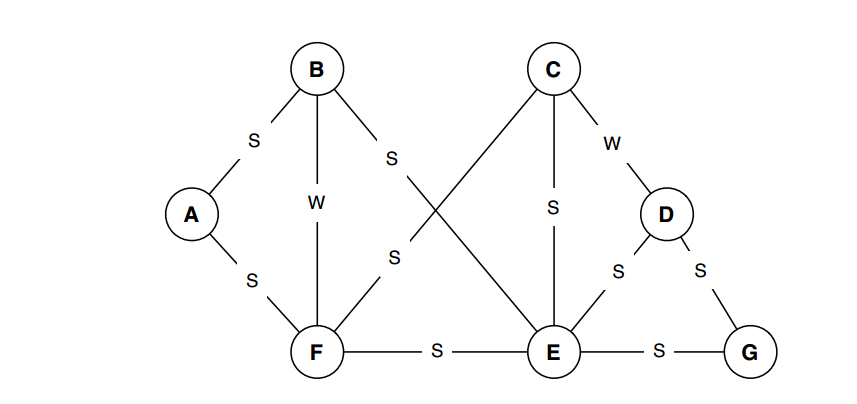
\includegraphics[width=15cm]{figures/figure1.png}
\caption{A simple figure.}
\label{fig:graph}
\end{figure}

Figures should always be placed at the top or bottom of the page they appear on (see Fig. \ref{fig:graph}).

\section{A Section that Contains a Table}

Numerical tables and compilations of data or facts in tabular form must be numbered consecutively. Each table must be labeled with a caption. Each caption should be unique so that two or more tables never share the same caption. The caption must be placed above the table, as it helps the reader to grasp the content of the table, even in the case of a long table running over several pages. Where applicable, the physical quantity listed must be indicated in the header of each column by a formula symbol or word and the corresponding unit.

Tables should always be placed at the top or bottom of the page they appear on or, as in this case, at the end of the section/chapter (see Table \ref{tab:xor}).

\begin{table}[ht!]
\center
\caption{A simple table.}
\begin{tabular}{cc|c}
A & B & A XOR B\\
\hline
0 & 0 & 0\\
0 & 1 & 1\\
1 & 0 & 1\\
1 & 1 & 0\\
\end{tabular}
\label{tab:xor}
\end{table}
\chapter{Methodology}\label{sec:Chapter3-Methodology}

This methodology chapter serves to introduce strategies, implementations, models and approaches which are put into practice in the Experiments chapter (Chapter~\ref{sec:Chapter4-Results}). Therefore, it will include:
\begin{itemize}[itemsep=0.1cm]
    \item \textbf{Particle Swarm Optimization:} an explanation of the most important of the sampling techniques utilized in the experiments.
    \item \textbf{Custom Implementation of PSO:} a detailed description of the design of the custom implementation of the algorithm, and some insights on the actual code implementation.
    \item \textbf{Enhancing Optuna Optimization:} a description of the design of the infrastructure built to run the experiments, in order to make Optuna more robust and reliable, and the experiments more comparable.
    \item \textbf{Applied Neural Network Models:} contains the list, with attached descriptions, of the machine learning objects involved in the experiments, along with descriptions of the training and evaluation of the utilized models.
\end{itemize}

\myparagraph{Code Repository:}
All the implementation details listed throughout this chapter refer to the following repository: \cite{Repository-THESIS}.
The repository is divided into two main packages, \texttt{utils} and \texttt{experiments}.
\\[0.3cm]The \texttt{experiments} package contains the code for the execution of the actual experiments and additional “private” code which is specific for the execution of the determined experiment.
\\[0.3cm]The \texttt{utils} package contains code which is common to all the experiments, in order to make the project more maintainable and modularized.

\section{Particle Swarm Optimization}

\subsection{Introduction to Particle Swarm Optimization}

Particle Swarm Optimization (PSO) is an optimization approach originally proposed by Kennedy and Eberhart in 1995 \cite{Tesi-3.3}. The idea was to replicate the behaviour of certain animal species which moves in groups, such as flocks of birds or shoals of fish.
\\[0.3cm]The reason is the assumption that each singular individual in the group can take advantage from the collective experience of the entire group; basically, each individual can benefit from what it learns from other individuals, and in the same way, it can share its discoveries with the other individuals \cite{Tesi-3.1}.

\subsubsection{Particle Swarm Optimization as an Optimization Problem}

Translating the previous explained behaviour into specific terms, each individual can be interpreted as an agent which “flies” in the Search Space, where each physical position is a candidate solution in the n-dimensional Search Space, and the best solution found by the entire group is the best solution.
\\[0.3cm]The best solution found by the entire group is likely not the real global optimal solution. However, it is a solution that is near the global optimum.
% 
% \myparagraph{Formalization of Particle Swarm Optimization:}
\\[0.3cm]The goal of Particle Swarm Optimization, as all optimization problems, is to find value which maximizes (or minimizes) the value of an objective (or Fitness) function $f$.
\\[0.3cm]The Objective Function $f$ is defined on a Search Space {$\textbf{X}$}, the multi-dimensional vector representing all the possible solutions within the defined limits.
The PSO algorithm will return the vector $X$, which represents a single solution, which maximizes (or minimizes) the value of $f$.
% 
% \myparagraph{General Procedure of PSO:}
\\[0.3cm]To find the maximum (or minimum) of the Fitness function $f$, the best solution would be to perform an exhaustive search on all the possible solutions. However, this approach is too computationally expensive, and basically inapplicable to higher-dimensional spaces \cite{Tesi-3.1}.
\\[0.3cm]Therefore, in PSO, the same way as a flock of birds searches for food, moving in the air, the algorithm starts with a number of random points in the search space, which are called Particles, and has them look for an optimal value by roaming in random directions.
\\[0.3cm]At each atomic step, each Particle (individual) searches for its Local Optimal value, basing its research on both the current Local Optimum, and the current Global Optimum of the whole Swarm.
After a certain number of iterations, the maximum (or minimum) value found as the Global Optimum is considered the optimal value for the function $f$.

\subsubsection{Particle Swarm Optimization Algorithm}

At the start of each iteration, each Particle has a position $x_i(t)$ and a velocity $v_i(t)$.

\myparagraph{Update of Particles:}\label{sec:UpdateOfParticles-3.1.1}
At the subsequent iteration, the update function will update the position and velocity of a Particle in accordance with the following rules:
\begin{equation}
	v_i(t+1) = \alpha v_i(t) + \beta_1(x_i^{(local)}(t) - x_i(t)) + \beta_2(x^{(global)}(t) - x_i(t))
\end{equation}
\begin{equation}
	x_i(t+1) = x_i(t) + v_i(t)
\end{equation}
Parameter $\alpha$ represents an “inertia”, which decreases over time, that is when t increases.
\\[0.3cm]Parameters $\beta_1$ and $\beta_2$, are the weight assigned to the Local and Global “parts” respectively. They are usually chosen randomly at each step. They are called Cognitive Coefficient and Social Coefficient, respectively.
\\[0.3cm]Parameter  $x_i^{(local)}$  is the Local Memory of an individual (Particle), it represents the best coordinates in the Search Space visited by that individual. It is updated as follows:
\begin{equation}
	x_i^{(local)} = x_i(\arg \max f(x_i(u)))
\end{equation}
Parameter $x^{(global)}$ is the Global Memory of the Swarm, it represents the best coordinates in the Search Space visited by an individual in the Swarm, basically the best solution so far. It is updated as follows:
\begin{equation}
	x^{(global)}(t) = x_j^{(local)}(t)
\end{equation}
Whenever Local Optimum (for each Particle) and Global Optimum (for the whole Swarm) is found, the values of the two memories are updated.

\myparagraph{Advantages of PSO Algorithm:}
Differently from other more traditional optimization algorithms, PSO does not depend on the gradient of the objective function.
Basically, unlike Gradient Descent, the movement of a Particle does not depend on which direction is “uphill” or “downhill”, because the Particle is guided by Local Optimum and Global Optimum only.
\\[0.3cm]This advantage makes PSO algorithms suitable for problems which objective functions are non-differentiable. Thus, it is an algorithm appliable to a wider range of optimization problems.
Another advantage is that PSO is an “Embarrassingly Parallel” problem; a type of problem particularly easy to parallelize, as each particle can be updated in parallel.

\myparagraph{Visual Example of PSO:}
In the figure (Fig.~\ref{fig:figure-3.1.1}), it can be observed how the particles progressively converge towards the Global Optimum, which represents the best solution found by the whole Swarm.
\begin{figure}[t]
	\centering
	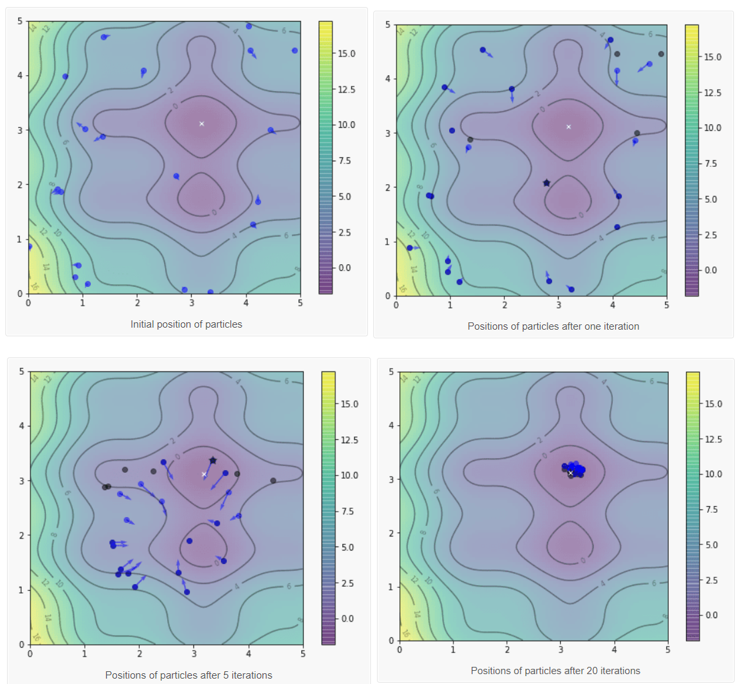
\includegraphics[width=14cm]{figures/figure-3.1.1.png}
	\caption[Visual Representation of Particle Swarm Optimization]{Visual representation of the convergence of the Particles to the Global Optimum in the Search Space in a Particle Swarm Optimization Algorithm. Source:~\cite{Tesi-3.1}}
	\label{fig:figure-3.1.1}
\end{figure}

\subsection{Components of Particle Swarm Optimization}

Particle Swarm Optimization can have better results, be faster and cheaper compared to other methods. It is an easy problem to parallelize. Does not require the target function to be differentiable. It has few and not very complex hyperparameters.
\\[0.3cm]In short, PSO has a large set of advantages; it is a modern solution to perform optimization tasks. The final objective remains the same as for every optimization problem: to minimize (or maximize) a given function.
\\[0.3cm]The three components of PSO algorithm are: Particle, Swarm and Optimization.

\subsubsection{Particle}

The Particle Swarm Optimization is inspired by the behaviour of flocks of birds. Therefore, the term “Particle”, refers to a single individual in the Swarm.
\\[0.3cm]Every Particle is defined by its Position and its Velocity in the Search Space.
The Position in the Search Space allows for the evaluation of the values corresponding to that position, whereas the Velocity allows Particles to move stochastically in the Search Space, in search of new better positions, and thus solutions.
% 
% \myparagraph{Initialization of Particles:}
\\[0.3cm]At the start of the optimization process, the positions of the Particles are defined randomly: random values of the Search Space are assigned to the Particles.
The Velocity and direction of the Particles are also randomly generated.
% 
% \myparagraph{Evaluation of Particles:}
\\[0.3cm]The Particle in the PSO is thus an agent, the position this agent has in the Search Space is a potential solution, a candidate solution.
Each Particle has Fitness values, which are evaluated by the Fitness Function, which is the function subject of the optimization.
The Fitness Function evaluates a Particle's Positions, taking in input the values of the Search Space corresponding to that position.

\subsubsection{Swarm}
The Swarm is the Population of Particles in the optimization process, it represents the flock of birds.
\\[0.3cm]PSO has similarities with Genetic Algorithms, but differently from them, there are no Evolution Operators to update the individual for the next generation.
In PSO the next generation of individuals is an update of the former generation, which Position and Velocity are updated in order to improve the Fitness.

\myparagraph{Inertia, Cognitive Intuition and Social Intuition:}
After each iteration in the Search Space, the Velocity of each Particle is stochastically accelerated; consequently, also its Position will change.
\\[0.3cm]The value the Velocity is going to be updated into is influenced by three factors: Inertia, Cognitive Intuition and Social Intuition. (Fig.~\ref{fig:figure-3.1.2})
\\[0.3cm]Inertia is the tendency to keep the Velocity from the previous iteration.
Cognitive Intuition is what makes the Particle accelerate toward the previous best Local Position, which is the best Position (corresponding to best Fitness) that Particle has achieved so far.
Social Intuition is what makes the Particle accelerate toward the previous best Global Position, which is the best Position (corresponding to best Fitness) the Particles in the Swarm have achieved so far.
\begin{figure}[t]
	\centering
	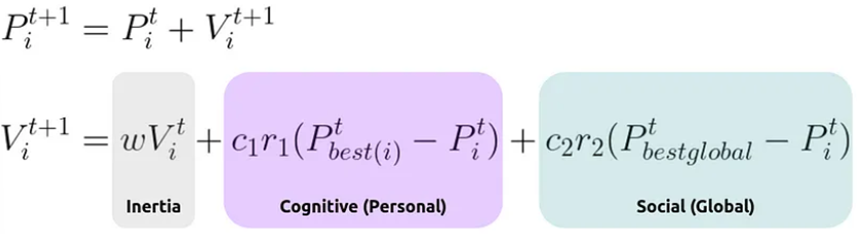
\includegraphics[width=13cm]{figures/figure-3.1.2.png}
	\caption[Alternative Update Functions for PSO]{Alternative update functions for the Velocity of the Particles in a Particle Swarm Optimization Algorithm, where the three components of the update function are represented, and additional parameters, $c_1$ and $c_2$ are introduced. Source:~\cite{Tesi-3.2}}
	\label{fig:figure-3.1.2}
\end{figure}

\subsubsection{Optimization}

The Optimization component of PSO, consists in the actual process of updating the parameters, with the correlated setting of Hyperparameters.
Inertia, Cognitive and Social coefficients have the function to control the levels of Exploitation and Exploration.
\\[0.3cm]Exploitation means using the good solutions found so far in order to search for even better solutions in that mathematical neighbourhood. Exploration means to explore distant sections of the Search Space, in search of new information on the Space or potentially improving solutions.
% 
% \myparagraph{Weighting of Acceleration:}
\\[0.3cm]At each iteration, both the Cognitive section and the Social section of the update formula are weighted by random terms \cite{Tesi-3.2} \cite{Tesi-3.5}.
Basically, Cognitive acceleration and Social acceleration are stochastically adjusted by weights to make the update process more random and less deterministic. The possible values that the coefficients can assume are in Fig.~\ref{fig:figure-3.1.3}.
\begin{figure}[t]
	\centering
	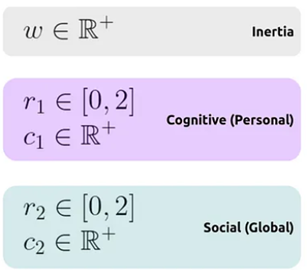
\includegraphics[width=5cm]{figures/figure-3.1.3.png}
	\caption[Values Ranges for PSO Parameters]{Ranges of values for the Parameters of a Particle Swarm Optimization Algorithm. Source:~\cite{Tesi-3.2}}
	\label{fig:figure-3.1.3}
\end{figure}
% 
% \myparagraph{Value of Inertia:}
\\[0.3cm]The value of the Inertia coefficient defines the ability of the Swarm to change direction.
Lower values of Inertia coefficient lead to better convergence; so low Inertia increases the exploitation of the best solutions.
Higher values of Inertia coefficient increase the exploration around the best solutions.
Values too high for Inertia, values $>1$, cause divergence of the Particles \cite{Tesi-3.2}.
% 
% \myparagraph{Value of Cognitive Coefficient:}
\\[0.3cm]The value of Cognitive coefficient defines the ability of the Swarm to be influenced by the personal solutions of each Particle.
If the Cognitive coefficient is too high, then there will be no convergence, as each individual would be too focused on its optimal solution \cite{Tesi-3.2}.
% 
% \myparagraph{Value of Social Coefficient:}
\\[0.3cm]The value of Social coefficient defines the ability of the Swarm to be influenced by the best global solutions of the whole Swarm.

\myparagraph{Auto Hyperparameters:}
Inertia, Cognitive and Social coefficients are all three Hyperparameters for the optimization process of PSO.
\\[0.3cm]Searching for the optimal values of their coefficient is a complex and expensive task, as it would require another optimization process.
Moreover, the optimal value of these parameters changes during the optimization process, as the iterations go on.
\\[0.3cm]Therefore, a satisfactory solution is to update the coefficients over the iterations \cite{Tesi-3.2}.
Good recommended update formulas, coming from empirical studies, are the equations below.
\\[0.3cm]The initial values should guarantee high exploration and more individuality, so high Inertia and Cognitive and low Social.
\\[0.3cm]Toward the end of the optimization, values should guarantee high exploitation and convergence to the local optimum, so low Inertia and Cognitive and high Social.
\begin{equation}
	w = 0.4\frac{(t-N)}{N^2} + 0.4
\end{equation}
\begin{equation}
	c_1 = -3\frac{t}{N} + 3.5
\end{equation}
\begin{equation}
	c_2 = +3\frac{t}{N} + 0.5
\end{equation}

\subsection{Principles, Applications and Variants of PSO}

This subsection, will examine: Principles of Swarm Intelligence, real-world applications of Particle Swarm Optimization, and PSO variants.

\subsubsection{Principles of Particle Swarm Optimization}

Particle Swarm Optimization has evolved a lot during its first experimental phase.
While it was originally meant to simulate the behaviour of a flock of birds, the final form of the algorithm resembles more of a Swarm than a flock. For this reason, it took the name of Swarm Optimization.
\\[0.3cm]The first researcher who talked about Swarm Intelligence, Millonas \cite{SwarmIntelligence}, defined five principles of Swarm Intelligence.
Particle Swarm Optimization adheres to all five principles.
\begin{enumerate}[itemsep=0.1cm]
    \item \textbf{Proximity Principle:} “The population should be able to perform simple space and time computations”.
	\item \textbf{Quality Principle:} “The population should be able to respond to quality factors in the environment”.
	The PSO adheres to this principle because the population, the Swarm, tends to follow the two positions Local Optimum and Global Optimum, which are the environment's factors.
	\item \textbf{Diverse Response Principle:} “The population should ensure enough diversity in its responses”.
	The PSO adheres to this principle because the responses range from the Local Optimum of the Particle and the Global Optimum of the Swarm, ensuring the diversity.
	\item \textbf{Stability Principle:} “The population should not change its behaviour at each environmental change”.
	The PSO adheres to this principle because the population only changes when the Global Optimum is updated and is therefore stable.
	\item \textbf{Adaptability Principle:} “The population should be able to change its behaviour when it is worth the computational price”.
	The PSO adheres to this principle because the population does change its behaviour when the Global Optimum is updated.
\end{enumerate}
% 
% \myparagraph{1 - Proximity Principle:}
% The population should be able to perform simple space and time computations.
% 
% \myparagraph{2 - Quality Principle:}
% The population should be able to respond to quality factors in the environment.
% \\[0.3cm]The PSO adheres to this principle because the population, the Swarm, tend to follow the positions Local Optimum and Global Optimum, which are the environment's factors.
% 
% \myparagraph{3 - Diverse Response Principle:}
% The population should ensure enough diversity in its responses.
% \\[0.3cm]The PSO adheres to this principle because the responses range from the Local Optimum of the Particle and Global Optimum of the Swarm, ensuring the diversity.
% 
% \myparagraph{4 - Stability Principle:}
% The population should not change its behaviour at each environmental change.
% \\[0.3cm]The PSO adheres to this principle because the population only changes when the Global Optimum is updated and is therefore stable.
% 
% \myparagraph{5 - Adaptability Principle:}
% The population should be able to change its behaviour when it Is worth the computational price.
% \\[0.3cm]The PSO adheres to this principle because the population does change its behaviour when the Global Optimum is updated.

\subsubsection{Applications of Particle Swarm Optimization}

One of the main reasons why Particle Swarm Optimization is widely used as optimization technique, is that it is well-suited to a wide range of problems \cite{Tesi-3.4}.
The advantage of PSO is that it has a small number of Hyperparameters to set, this allow the algorithm to be easily appliable to specific applications \cite{Tesi-3.4} \cite{Tesi-3.1} \cite{Tesi-3.3} \cite{Tesi-3.5}.
\begin{itemize}[itemsep=0.1cm]
    \item \textbf{Evolution of Neural Networks:} Particle Swarm Optimization can substitute traditional methods for the optimization of a Neural Network's weights.
	PSO is able to reach or outperform traditional approaches like Backpropagation.
	PSO can work so well with Neural Networks, that it can not only be used to optimize the networks' weights, but also their structure. PSO is effective for any network architecture \cite{Tesi-3.4}.
	\item \textbf{Human Tremor Diagnosis:} PSO has been used in combination with Neural Networks for the diagnosis of Humar Tremor conditions, for example, Parkison's Disease \cite{Tesi-3.4}.
	\item \textbf{End Milling Manufacturing:} PSO has been used in combination with Neural Networks for End Milling manufacturing \cite{Tesi-3.4}.
	\item \textbf{Voltage Stability:} PSO has been used for dynamic power and voltage control in a Japanese electric establishment \cite{Tesi-3.4}.
	\item \textbf{Determination of Battery State:} PSO has been used in combination with Neural Networks for estimating the state-of-charge of electrical or hybrid vehicles \cite{Tesi-3.4}.
\end{itemize}
% \\[0.3cm]\textbf{Evolution of Neural Networks:} Particle Swarm Optimization can substitute traditional methods for the optimization of a Neural Network weights.
% PSO is able to reach or outperform traditional approaches like Backpropagation.
% PSO can work so well with Neural Networks, that not only can be used to optimize the networks' weights, but also their structure. PSO applies is effective for any network architecture \cite{Tesi-3.4}.
% \\[0.3cm]\textbf{Human Tremor Diagnosis:} PSO has been used in combination with Neural Networks for the diagnosis of Humar Tremor conditions, for example Parkison's Disease \cite{Tesi-3.4}.
% \\[0.3cm]\textbf{End Milling Manufacturing:} PSO has been used in combination with Neural Networks for End Milling manufacturing \cite{Tesi-3.4}.
% \\[0.3cm]\textbf{Voltage Stability:} PSO has been used for a dynamic power and voltage control in a Japanese electric establishment \cite{Tesi-3.4}.
% \\[0.3cm]\textbf{Determination of Battery State:} PSO has been used in combination with Neural Networks for estimating the state-of-charge of electrical or hybrid vehicles \cite{Tesi-3.4}.

\subsubsection{Variants of Particle Swarm Optimization}

The Particle Swarm Optimization is a popular and effective optimization technique; therefore, many variants of the approach have been developed \cite{Tesi-3.2}.
\\[0.3cm]Variants primarily focus on adding evolutionary capabilities to PSO or improving performance with Hyperparameters.
\begin{itemize}[itemsep=0.1cm]
    \item \textbf{Hybrid of Genetic Algorithm and PSO (GA-PSO):} implements the main aspects of GA approach, such as the capability of breeding and crossover.
    \item \textbf{Hybrid of Evolutionary Programming and PSO (EPSO):} implements the tournament selection in PSO, where the losing Particles change their position.
    \item \textbf{Adaptive PSO (APSO):} applies Fuzzy Logic to the Inertia coefficient. In addition, uses another PSO to perform the Hyperparameter Optimization for the first PSO.
    \item \textbf{Multi Objective PSO (MOPSO):} implements the concept of Pareto Dominance to determine which Particle should set the Global Optimum \cite{Tesi-3.5}.
    \item \textbf{Discrete PSO (DPSO):} makes the performance of optimization better, for example using a mixed-search approach \cite{Tesi-3.5}.
\end{itemize}
% 
% \myparagraph{Hybrid of Genetic Algorithm and PSO (GA-PSO):}
% Hybrid of Genetic Algorithm and PSO (GA-PSO) implements the mainly aspects of GA approach as the capability of breeding and crossover.
% 
% \myparagraph{Hybrid of Evolutionary Programming and PSO (EPSO):}
% Hybrid of Evolutionary Programming and PSO (EPSO) implements the tournament selection in PSO, where the losing Particles changes their position.
% 
% \myparagraph{Adaptive PSO (APSO):}
% Adaptive PSO (APSO) applies Fuzzy Logic to the Inertia coefficient. In addition, uses another PSO to perform the Hyperparameter Optimization for the first PSO.
% 
% \myparagraph{Multi Objective PSO (MOPSO):}
% Multi Objective PSO (MOPSO) implements the concept of Pareto Dominance to determine which Particle should set the Global Optimum \cite{Tesi-3.5}.
% 
% \myparagraph{Discrete PSO (DPSO):}
% Discrete PSO (DPSO) makes the performance of optimization better, for example using mixed search approach \cite{Tesi-3.5}.

\section{Custom Implementation of PSO}\label{sec:CustomImplementationOfPSO-3.2}

Particle Swarm Optimization, as described in the last section, is a powerful and successful Optimization algorithm, that can also be applied to HPO.
In the last few years, many libraries for PSO have been developed, for instance, PySwarm, which is probably the most popular.
\\[0.3cm]The problem with these libraries, as for the objectives of the experiments, is that they are hardly customizable, and often lack in explainability, making them less adaptable to HPO.
While this problem of explainability is potentially fixable, without being able to customize the original algorithm, the experiments would not be scientifically comparable between the ones run using Optuna's samplers.
\\[0.3cm]Therefore, two potential solutions are proposed so as to apply PSO to an HPO problem: the first was to implement from scratch a PSO algorithm that follows the same style as Optuna so that the two would be comparable; the second was to implement an Optuna Sampler with PSO.
The implementation of an Optuna Sampler with PSO will be discussed in the next section. In this section it will be examined the design of the PSO algorithm from scratch.
\\[0.3cm]All the code mentioned in this section refers to the package\newline\texttt{/experiments/PSO\_experiment/backend/} of the code repository \cite{Repository-THESIS}.

\subsection{High-Level Design}

The components of the algorithm are divided into five Python files: \texttt{PSO.py},\newline\texttt{pso\_pruners.py}, \texttt{pso\_runner.py}, \texttt{pso\_train\_utils.py} and \texttt{pso\_utils.py}.
These code files contain only what the algorithm needs to work, meaning that they do not contain the actual code of the experiments. In fact, the algorithm code is designed to mimic the functioning of Optuna, so that the same code to set up the Optuna experiments can be used to set up and perform experiments with this implementation of PSO. (Class Diagram in Fig.~\ref{fig:figure-3.2.1})
% 
% \myparagraph{Contents of the Main Code Files:}
\\[0.3cm]The contents and purpose of the main code files are the following:
\begin{itemize}[itemsep=0.1cm]
    \item \texttt{PSO.py}: is the main file of the package, the actual core of the algorithm. It contains the \texttt{PSO} and \texttt{Particle} classes, together with some other private code.
    \item \texttt{pso\_pruners.py}: contains the definition of the Pruners of the mini library. At the current state there is only one implemented Pruner which is the Median Pruner. It mimics the functioning of Optuna's Pruners.
    \item \texttt{pso\_runner.py}: contains the definition of the \texttt{PSORunner} class, which is a wrapper of the optimization process that manages potential errors, logging, and saving of the results.
    \item \texttt{pso\_train\_utils.py}: contains the train loop function which should be used inside the objective function of the optimization process. It also contains some other private code.
    \item \texttt{pso\_utils.py}: contains some constants and utility functions, in particular the one applied to encode and decode the value of the Hyperparameters from “internal” to “external” representations and vice-versa.
\end{itemize}
\begin{figure}[t]
	\centering
	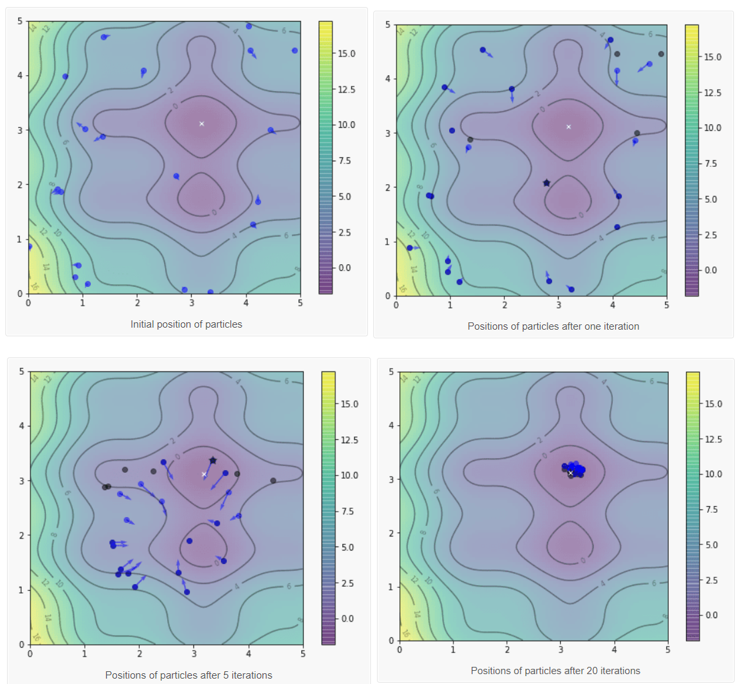
\includegraphics[width=15cm]{figures/figure-3.2.1.png}
	\caption[Class Diagram of Custom PSO Implementation]{Class Diagram of the custom implementation of the Particle Swarm Optimization with the related support code.}
	\label{fig:figure-3.2.1}
\end{figure}

\subsection{Components of the PSO Algorithm}

The true core of the algorithm, contained in \texttt{PSO.py}, consists of three fundamental components, which are: \texttt{Particle}, \texttt{PSOTrial} and \texttt{PSO}.

\subsubsection{Particle}

The \texttt{Particle} class is the representation of the concept of “Particle” in the original PSO algorithm.
% 
% \myparagraph{Attributes:}
\\[0.3cm]In this specific implementation, the Particle has the following attributes: \texttt{paticle\_id}, \texttt{position}, \texttt{velocity}, \texttt{personal\_best\_position}, \texttt{personal\_best\_score}.
The position and the velocity of the particle are initialized with randomly generated arrays.
% 
% \myparagraph{Methods:}
\\[0.3cm]The particle has two methods, which are \texttt{update\_velocity()} and \texttt{update\_position()}. 
The version of the strategy for the velocity update is the one with the Cognitive and the Social coefficients ($c_1$ and $c_2$). The random coefficients ($r_1$ and $r_2$) are chosen randomly, whereas, the other two coefficients, together with the Inertia coefficient ($w$), are passed as an input.
The strategy for the position update is the standard one, with the exception that values which go outside the Search Space are clipped (approximated to the nearest bound value).

\subsubsection{PSOTrial}

The \texttt{PSOTrial} class, as the name suggests, is a representation of a trial during the optimization. Its functioning is inspired by the \texttt{Trial} object of Optuna.
Its main objective is to carry metadata regarding each trial of the optimization process, so as to the results can be displayed the same way they are in Optuna.
% 
% \myparagraph{Attributes:}
\\[0.3cm]The \texttt{PSOTrial} object has the following attributes: \texttt{particle\_id}, \texttt{generation}, \newline\texttt{hyperparameters}, \texttt{datetime\_start}, \texttt{datetime\_complete}, \texttt{duration}, \texttt{score}, \texttt{state}, \texttt{user\_attrs}, \texttt{is\_pruned}, \texttt{pruner}, \texttt{last\_reported\_step}, \texttt{best\_reported\_score}.
The last four attributes are related to the pruning system. The \texttt{user\_attrs} attribute is a map object which allows the user to set custom metadata in the trial, like it can be done in Optuna. The other attributes are self-explainatory.
% 
% \myparagraph{Methods:}
\\[0.3cm]The methods realize functionalities such as completion of a trial, conversion to map, setters, and functions related to pruning.

\subsubsection{PSO}

The \texttt{PSO} class is the representation of the actual PSO algorithm. It is designed to be equivalent to a \texttt{Study} object of Optuna.
One instance of the \texttt{PSO} class carries on a whole optimization process, in the same way as an instance of Optuna's \texttt{Study} instance.
% 
% \myparagraph{Attributes:}
\\[0.3cm]The attributes of the \texttt{PSO} class are the following:
\begin{itemize}[itemsep=0.1cm]
    \item \texttt{objective\_function}: the objective function of the HPO process, to be passed at the initialization of the object just like in Optuna.
    \item \texttt{bounds}: is a 2D array which contains the lower bounds and the upper bounds of each non-categorical hyperparameter.
    \item \texttt{hps}: contains the mapping between the hyperparameter name and the index inside the inner arrays of bounds.
    \item \texttt{num\_particles}: is a hyperparameter of the algorithm itself; it represents the number of Particles in the Swarm.
    \item \texttt{max\_generations}: is another hyperparameter of the algorithm itself; it represents the maximum number of iterations (Generations) of the algorithm.
    \item \texttt{pruner}: the Pruner object to use in the algorithm.
    \item \texttt{pso\_stopper}: must be an \texttt{PSOStopper} object, which is another secondary class defined in the file. It Early-Stops the process according to a specified Tolerance and Patience.
    \item \texttt{swarm}: is the representation of the concept of Swarm. Rather than creating a specific class for it, it simply is a list of Particles (list of \texttt{Particle}).
    \item \texttt{global\_best\_score}: the best score at any given point in time.
    \item \texttt{global\_best\_position}: array which values represent the coordinates in the Search Space for the best position at any given point in time.
    \item \texttt{trials\_list}: list of all the \texttt{PSOTrial} objects.
    \item \texttt{best\_trial}: initialized at the end of the optimization, stores the best trial.
\end{itemize}
%
% \myparagraph{Methods:}
The methods of the \texttt{PSO} class, excluding the private or less important methods, are the following: \texttt{optimize()}, \texttt{inertia\_factor\_update()}, \texttt{cognitive\_factor\_update()}, \texttt{social\_factor\_update()}.
The three update methods are implemented using the formulas explained in the Particle Swarm Optimization section (Sec.~\ref{sec:UpdateOfParticles-3.1.1}).
\\[0.3cm]The \texttt{optimize()} method is where the actual PSO algorithm takes place. Here is where the optimization loop happens. The first level loop iterates over the maximum number of generations, then the inner loop iterates over each particle of the swarm.
After the particle is evaluated during a determined generation, and thus in a determined position, two checks are made to determine if the current result is better than the local and global better results.
Finally, at the end of a generation, each particle is updated using its update methods, with the values for $w$, $c_1$ and $c_2$ obtained from the three update methods mentioned earlier.
At the end of the whole loop, the method ends, returning the best global hyperparameters and the best global score.

\section{Enhancing Optuna Optimization}\label{sec:EnhancingOptuna-3.3}

Hyperparameter Optimization is expensive, and tools like Optuna not only exist to make the process more efficient but also to simplify the setup of the optimization.
Nevertheless, especially when the experiments grow in complexity, even tools like Optuna start to show weaknesses and robustness problems.
\\[0.3cm]Therefore, it is necessary to use Optuna to its full potential, gaining advantage from its additional abilities, such as the Storage. Moreover, an infrastructure beyond Optuna is also necessary to handle error throwing and to make persistent the data that Optuna Storage does not memorize.
\\[0.3cm]These extras are not always easy to setup, or at least require a setup for each Study. This, added to the already present normal setup of the Study, with the creation of the object and the launch of the optimization, makes the Study initialization process very heavy.
This would be perfectly fine in normal circumstances, but the goal of the proposed experiments, is to compare the different optimization techniques and sampling algorithms, thus, the previously described workflow should be repeated for each Study.
\\[0.3cm]The solution is to abstract some functionalities of Optuna, basically wrapping them, so as to reduce the quantity of code to write and improve the performance and reliability of the processes. (Object Diagram in Fig.~\ref{fig:figure-3.3.1})
\\[0.3cm]All the code mentioned in this section refers to the package \texttt{/utils/} of the code repository \cite{Repository-THESIS}.
\begin{figure}[t]
	\centering
	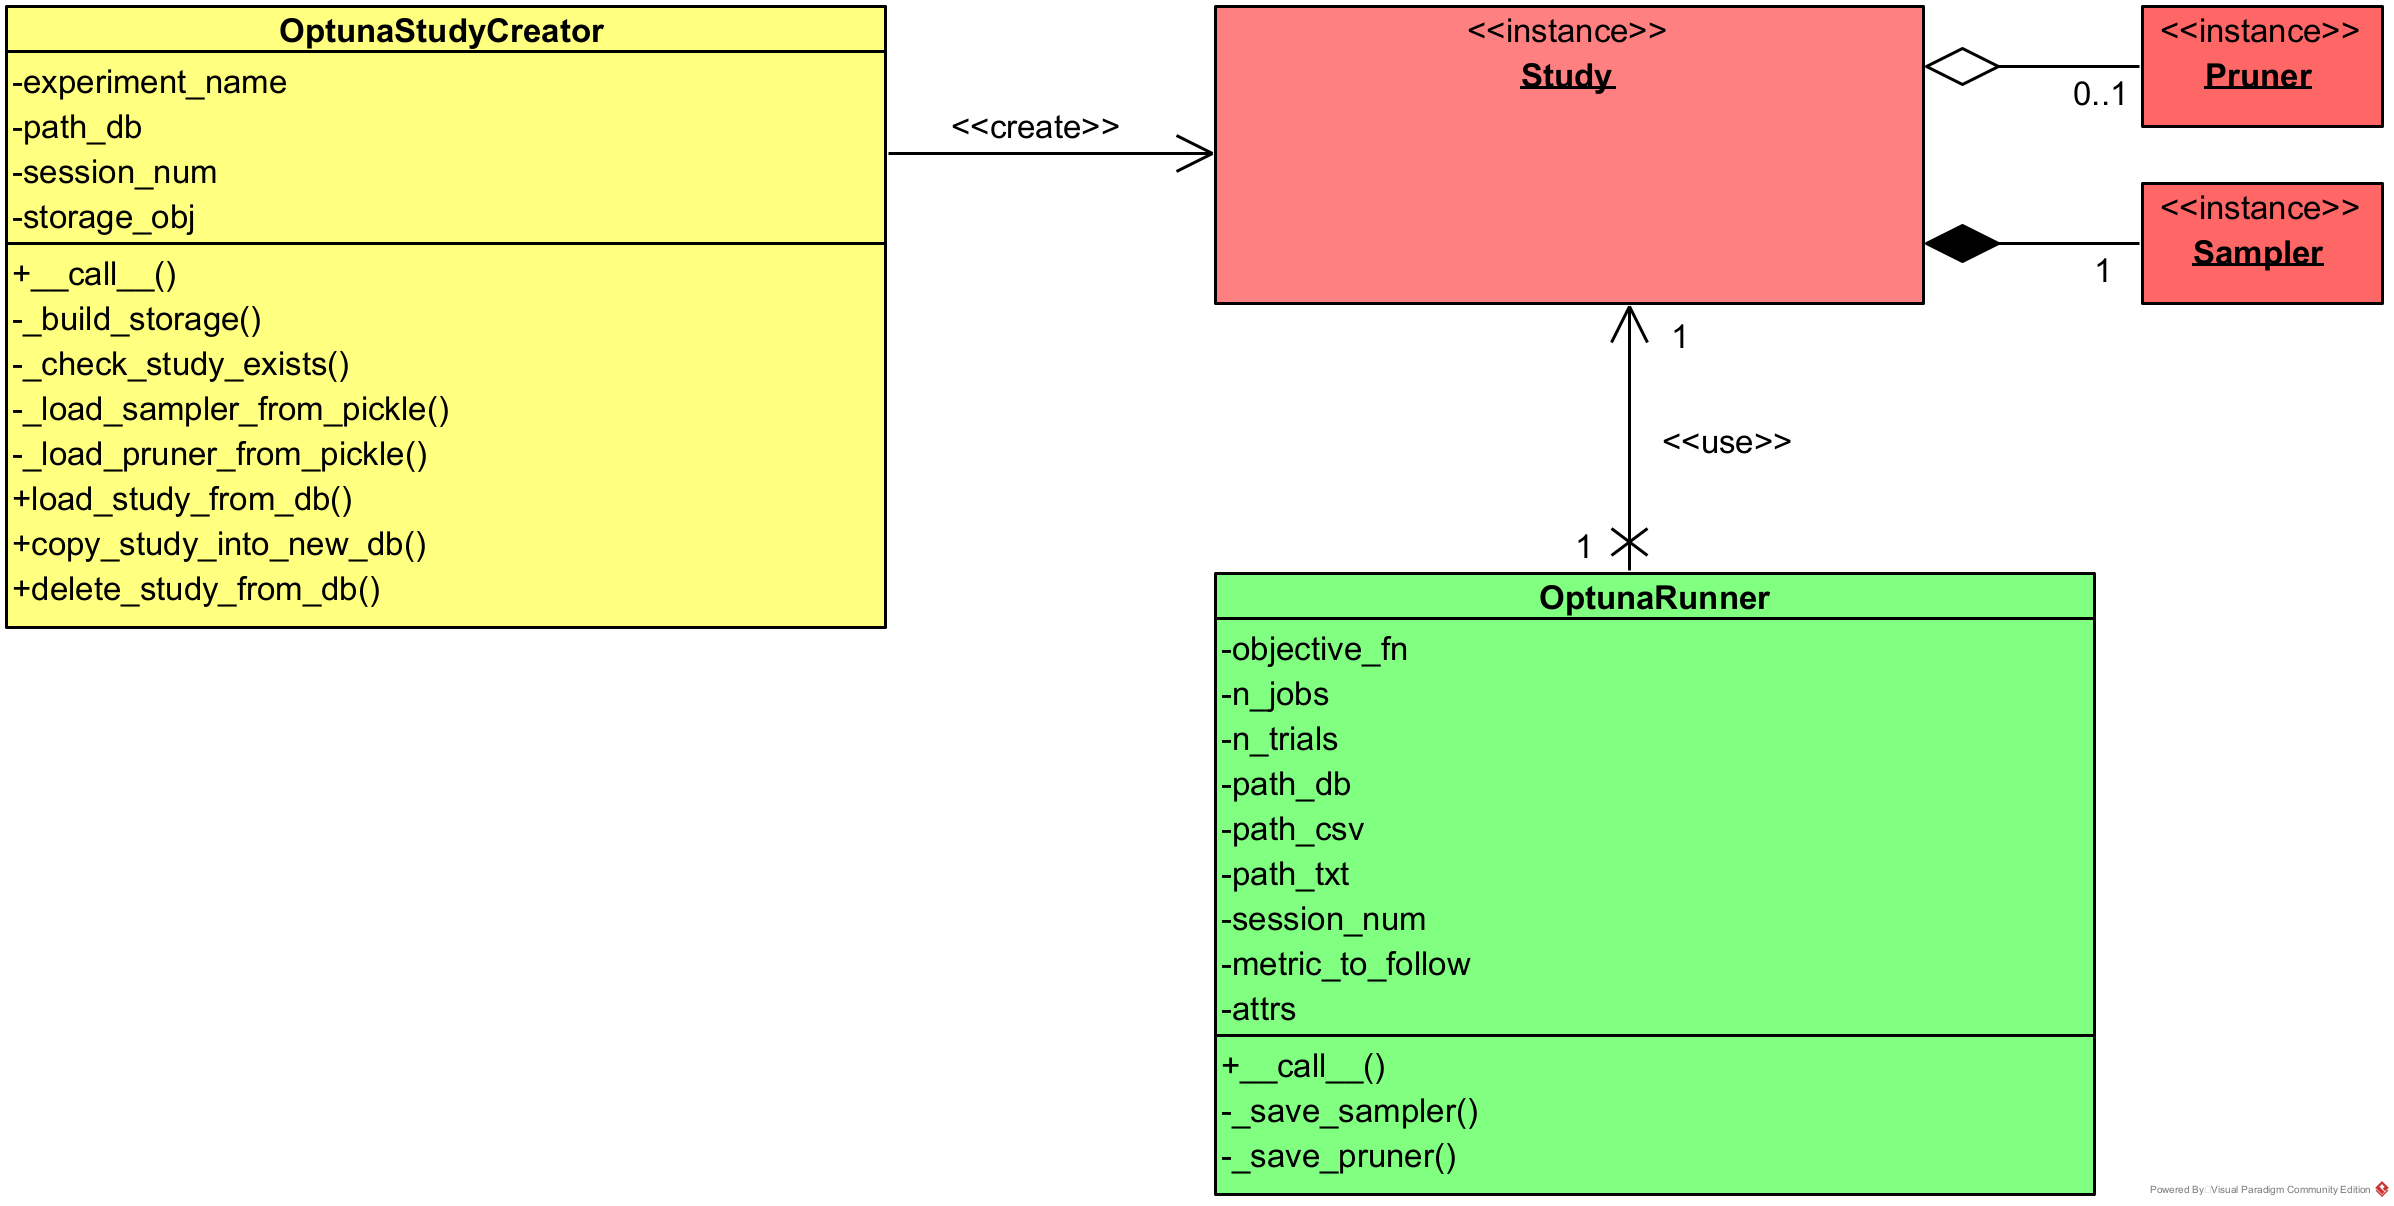
\includegraphics[width=15cm]{figures/figure-3.3.1.png}
	\caption[Object Diagram of Optuna Wrapping]{Object Diagram of the “wrapping”, or enhancement, of Optuna functionalities.}
	\label{fig:figure-3.3.1}
\end{figure}

\subsection{Optuna Wrapping}

The two main concerns relative to the abstraction of Optuna's functionalities are the initialization of the Study and the running of the optimization.
The proposed infrastructure, which wraps those two functionalities, has various objectives: to implement persistency (for both Optuna and additional metadata such as logs), to handle errors, to save the execution state of samplers and pruners (which Optuna does not do natively), to log and save the results in various formats, and other capabilities (like copying a Study to another DB, loading a Study from a DB, deleting a Study).
\\[0.3cm]As a result, by abstracting the process of creation and run of the optimization, the code is totally reusable for each Sampler, therefore making each singular experiment comparable to one another.
\\[0.3cm]The main files of the wrapping are \texttt{optuna\_study\_creator.py} and \texttt{optuna\_runner.py}.

\subsubsection{Optuna Study Creator}

Contained in the file \texttt{optuna\_study\_creator.py}, the class \texttt{OptunaStudyCreator} abstracts the process of creation of one single Study representing the optimization experiment.
% 
% \myparagraph{Creating the Study:}
\\[0.3cm]After initializing the object with values which will be common for all the studies, by calling it, it is possible to create new \texttt{Study} objects.
In particular the creator checks if the DB is present at all, checks if the study is already present in the DB, initializes the DB, initializes the Study representation in the DB, defines the storage object (which is the connection between the Study and its database).
In case the Study needs to be loaded, the creator also checks if there are pruners or samplers' states saved and eventually loads them into the optimization process.
% 
% \myparagraph{Additional Functionalities:}
\\[0.3cm]The class also contains methods to copy a Study to another DB, load a study from another DB and delete a Study from a DB.

\subsubsection{Optuna Runner}

Contained in the file \texttt{optuna\_runner.py}, the class \texttt{OptunaRunner} abstracts the process of optimization of one single Study representing the optimization experiment.
% 
% \myparagraph{Running the Study:}
\\[0.3cm]After initializing the object with values which will be common for all the studies, by calling it and passing the \texttt{Study} as input, it is possible to run the Study, equivalently to the \texttt{optimize()} method of Optuna.
The runner checks if there is any log file already present, creates the log file, runs the optimization, catches exceptions, saves the execution state of the Sampler and the Pruner of the Study, logs and saves the results of the optimization experiment.

\subsubsection{Other Optuna-Related Code}

As mentioned earlier, the proposed experiments create and run multiple optimizations, therefore, in addition to the strategies explained so far, another part of the code which needs to be as much standardized and abstract as possible is the Objective Function.
\\[0.3cm]The following files in the \texttt{/utils/} package contain code that helps with this.
\begin{itemize}[itemsep=0.1cm]
    \item \texttt{train\_loop.py}: contains the function that executes the training of the model object of the trial. Inside the loop are also defined the instructions related to pruning, early stopping, logging, and data persistence.
    \item \texttt{early\_stopper.py}: contains the definition of the \texttt{EarlyStopper} object, utilized to early-stop training loops within a trial which are no longer improving.
    \item \texttt{regularizer.py}: contains the definition of the \texttt{Regularizer} object, utilized for the Regularization in the experiments.
    \item \texttt{logger.py}: contains the definition of the \texttt{Logger} object, which is used throughout the whole optimization process to memorize debug information, errors, warnings, and logging information.
    \item \texttt{file\_name\_builder.py}: contains utils functions to create folders and filenames for the files of logging or persistence in general (such else results files).
    \item \texttt{build\_dateset.py}: contains functions that abstract the creation of the dataset, regardless of the particular experiment.
    \item \texttt{build\_dataloader.py}: contains functions that abstract the creation of the data loaders, regardless of the particular experiment.
    \item \texttt{model\_utils.py}: arguably the most important of this list, contains various functions, called in the objective function, which allow to initialize the components of the optimization (Loss Function, Model HPs, Training HPs) using the converted values of HPs sampled by Optuna.
\end{itemize}
% 
% \myparagraph{train\_loop.py:}
% Contains the function which executes the training of the model object of the trial. Inside the loop are also defined the instructions related to pruning, early stopping, logging and data persistence.
% 
% \myparagraph{early\_stopper.py:}
% Contains the definition of the \texttt{EarlyStopper} object, utilized to early stop training loops within a trial which are no longer improving.
% 
% \myparagraph{regularizer.py:}
% Contains the definition of the \texttt{Regularizer} object, utilized for the Regularization in the experiments.
% 
% \myparagraph{logger.py:}
% Contains the definition of the \texttt{Logger} object, which is used throughout the whole optimization to process to memorize debug information, errors, warnings, and logging information.
% 
% \myparagraph{file\_name\_builder.py:}
% Contains utils functions to create folders and name for the files of logging or persistence in general (also include the results files).
% 
% \myparagraph{build\_dateset.py:}
% Contains functions that abstract the creation of the dataset, regardless of the experiment.
% 
% \myparagraph{build\_dataloader.py:}
% Contains functions that abstract the creation of the data loaders, regardless of the experiment.
% 
% \myparagraph{model\_utils.py:}
% Arguably the most important of this list, contains various functions, called in the objective function, which allow to initialize the components of the optimization (Loss Function, Model HPs, Training HPs) using the converted values sampled of HPs sampler by Optuna.

\subsection{Custom Optuna PSO Sampler}\label{sec:CustomOptunaPSOSampler-3.3.2}
As mentioned in the section of the Custom PSO Implementation (Sec.~\ref{sec:CustomImplementationOfPSO-3.2}), one alternative approach to HPO using PSO was to integrate a PSO algorithm in Optuna as a Sampler.
\\[0.3cm]Optuna allows developers to define new Samplers. In order to do this, the custom sampler should inherit from the class \texttt{BaseSampler} of Optuna and override some methods.
\\[0.3cm]The code described in this section refers to the \texttt{/utils/optuna\_utils/pso\_sampler.py} file of the code repository \cite{Repository-THESIS}.

\subsubsection{Initialization}
The Sampler requires two initialization parameters, which are the number of particles, and the number of generations. 
Even if, in the current state of the implementation, there are no integrity checks, these values should be compatible with the number of trials to execute, which is a parameter of the Study running function of Optuna. 
\\[0.3cm]As soon as the first trial starts, the Swarm is initialized; it is a list of Particles, where a Particle is defined in the same exact way described in the section of Custom Implementation of PSO (Sec.~\ref{sec:CustomImplementationOfPSO-3.2}).
\\[0.3cm]Until a trial is completed or pruned, Optuna calls the \texttt{sample\_indipendent()} method, which samples the value for the hyperparameters randomly with a \texttt{RandomSampler}.
\\[0.3cm]After the completion of the first trial, the Search Space is also initialized. The Search Space cannot be initialized earlier by Optuna because the current possible value ranges of the Hyperparameters are unknown to Optuna before running the Objective Function at least once.
\\[0.3cm]The Sequence Diagram of the \texttt{BaseSampler} (Fig.~\ref{fig:figure-3.3.1}) allows to understand how the \texttt{PSOSampler} interacts with the rest of the Optuna components and executes the sampling.
\begin{figure}[H]
	\centering
	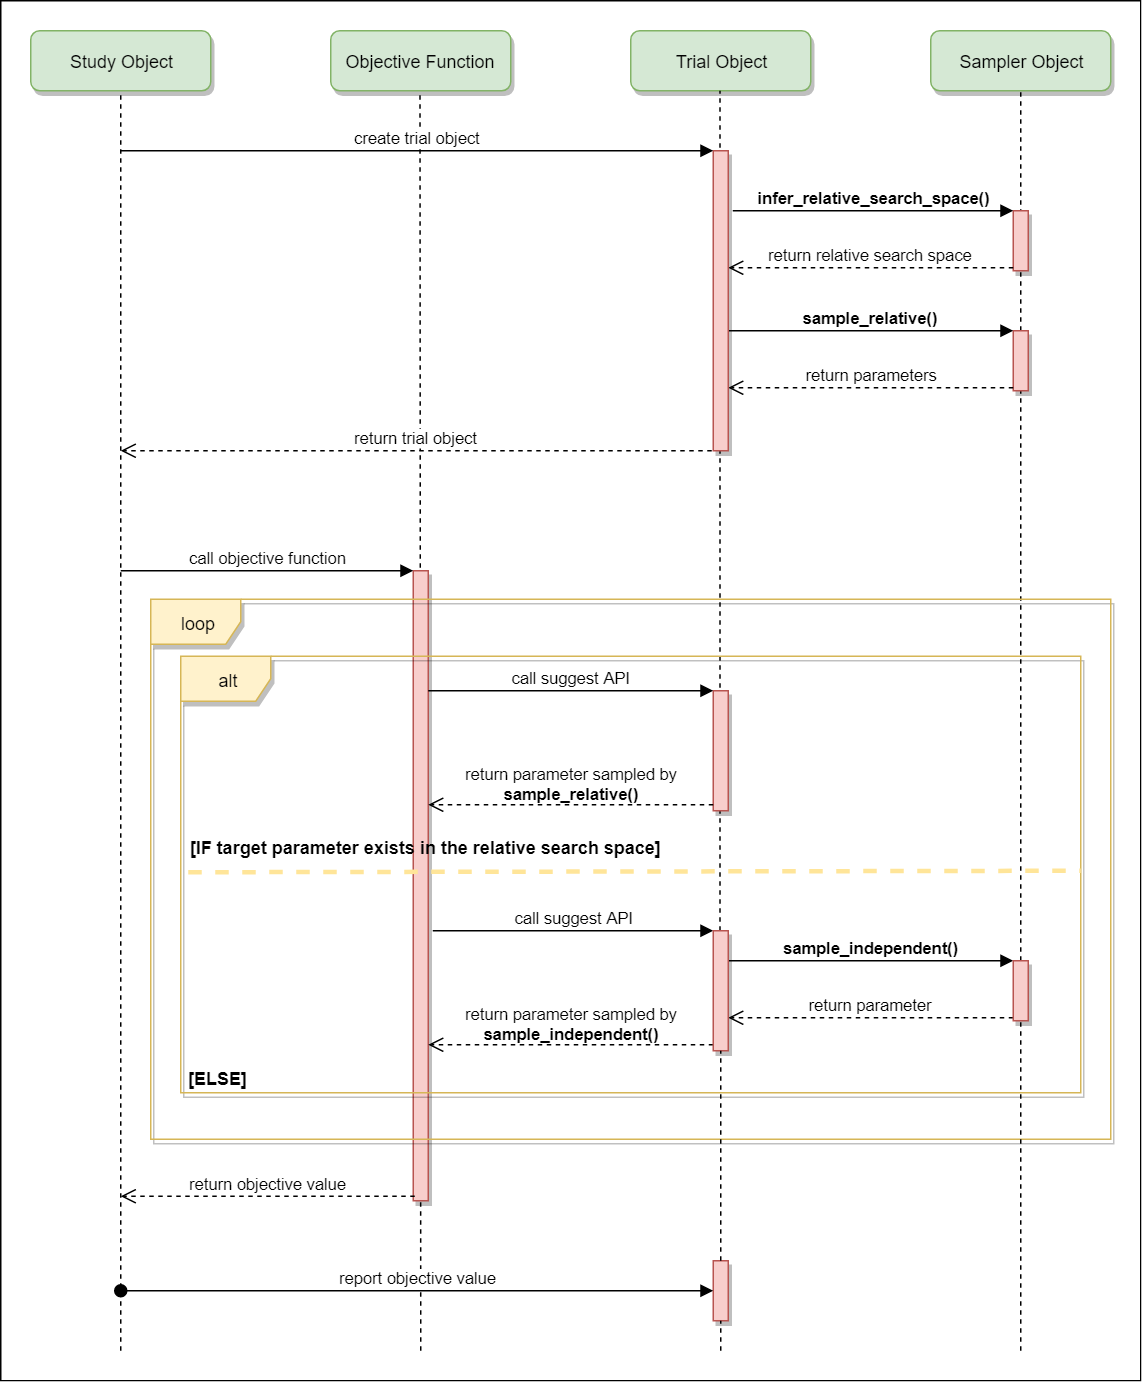
\includegraphics[width=15cm]{figures/figure-3.3.2.png}
	\caption[Sequence Diagram of Optuna's Samplers]{Sequence Diagram of the interaction between Optuna's Samplers and the rest of the Optuna's components. Through the diagram, is possibile to understand how a sampler in Optuna behaves at the start of a Trial. Source: \cite{Optuna}}
	\label{fig:figure-3.3.2}
\end{figure}
% \begin{figure}[t]
% 	\centering
% 	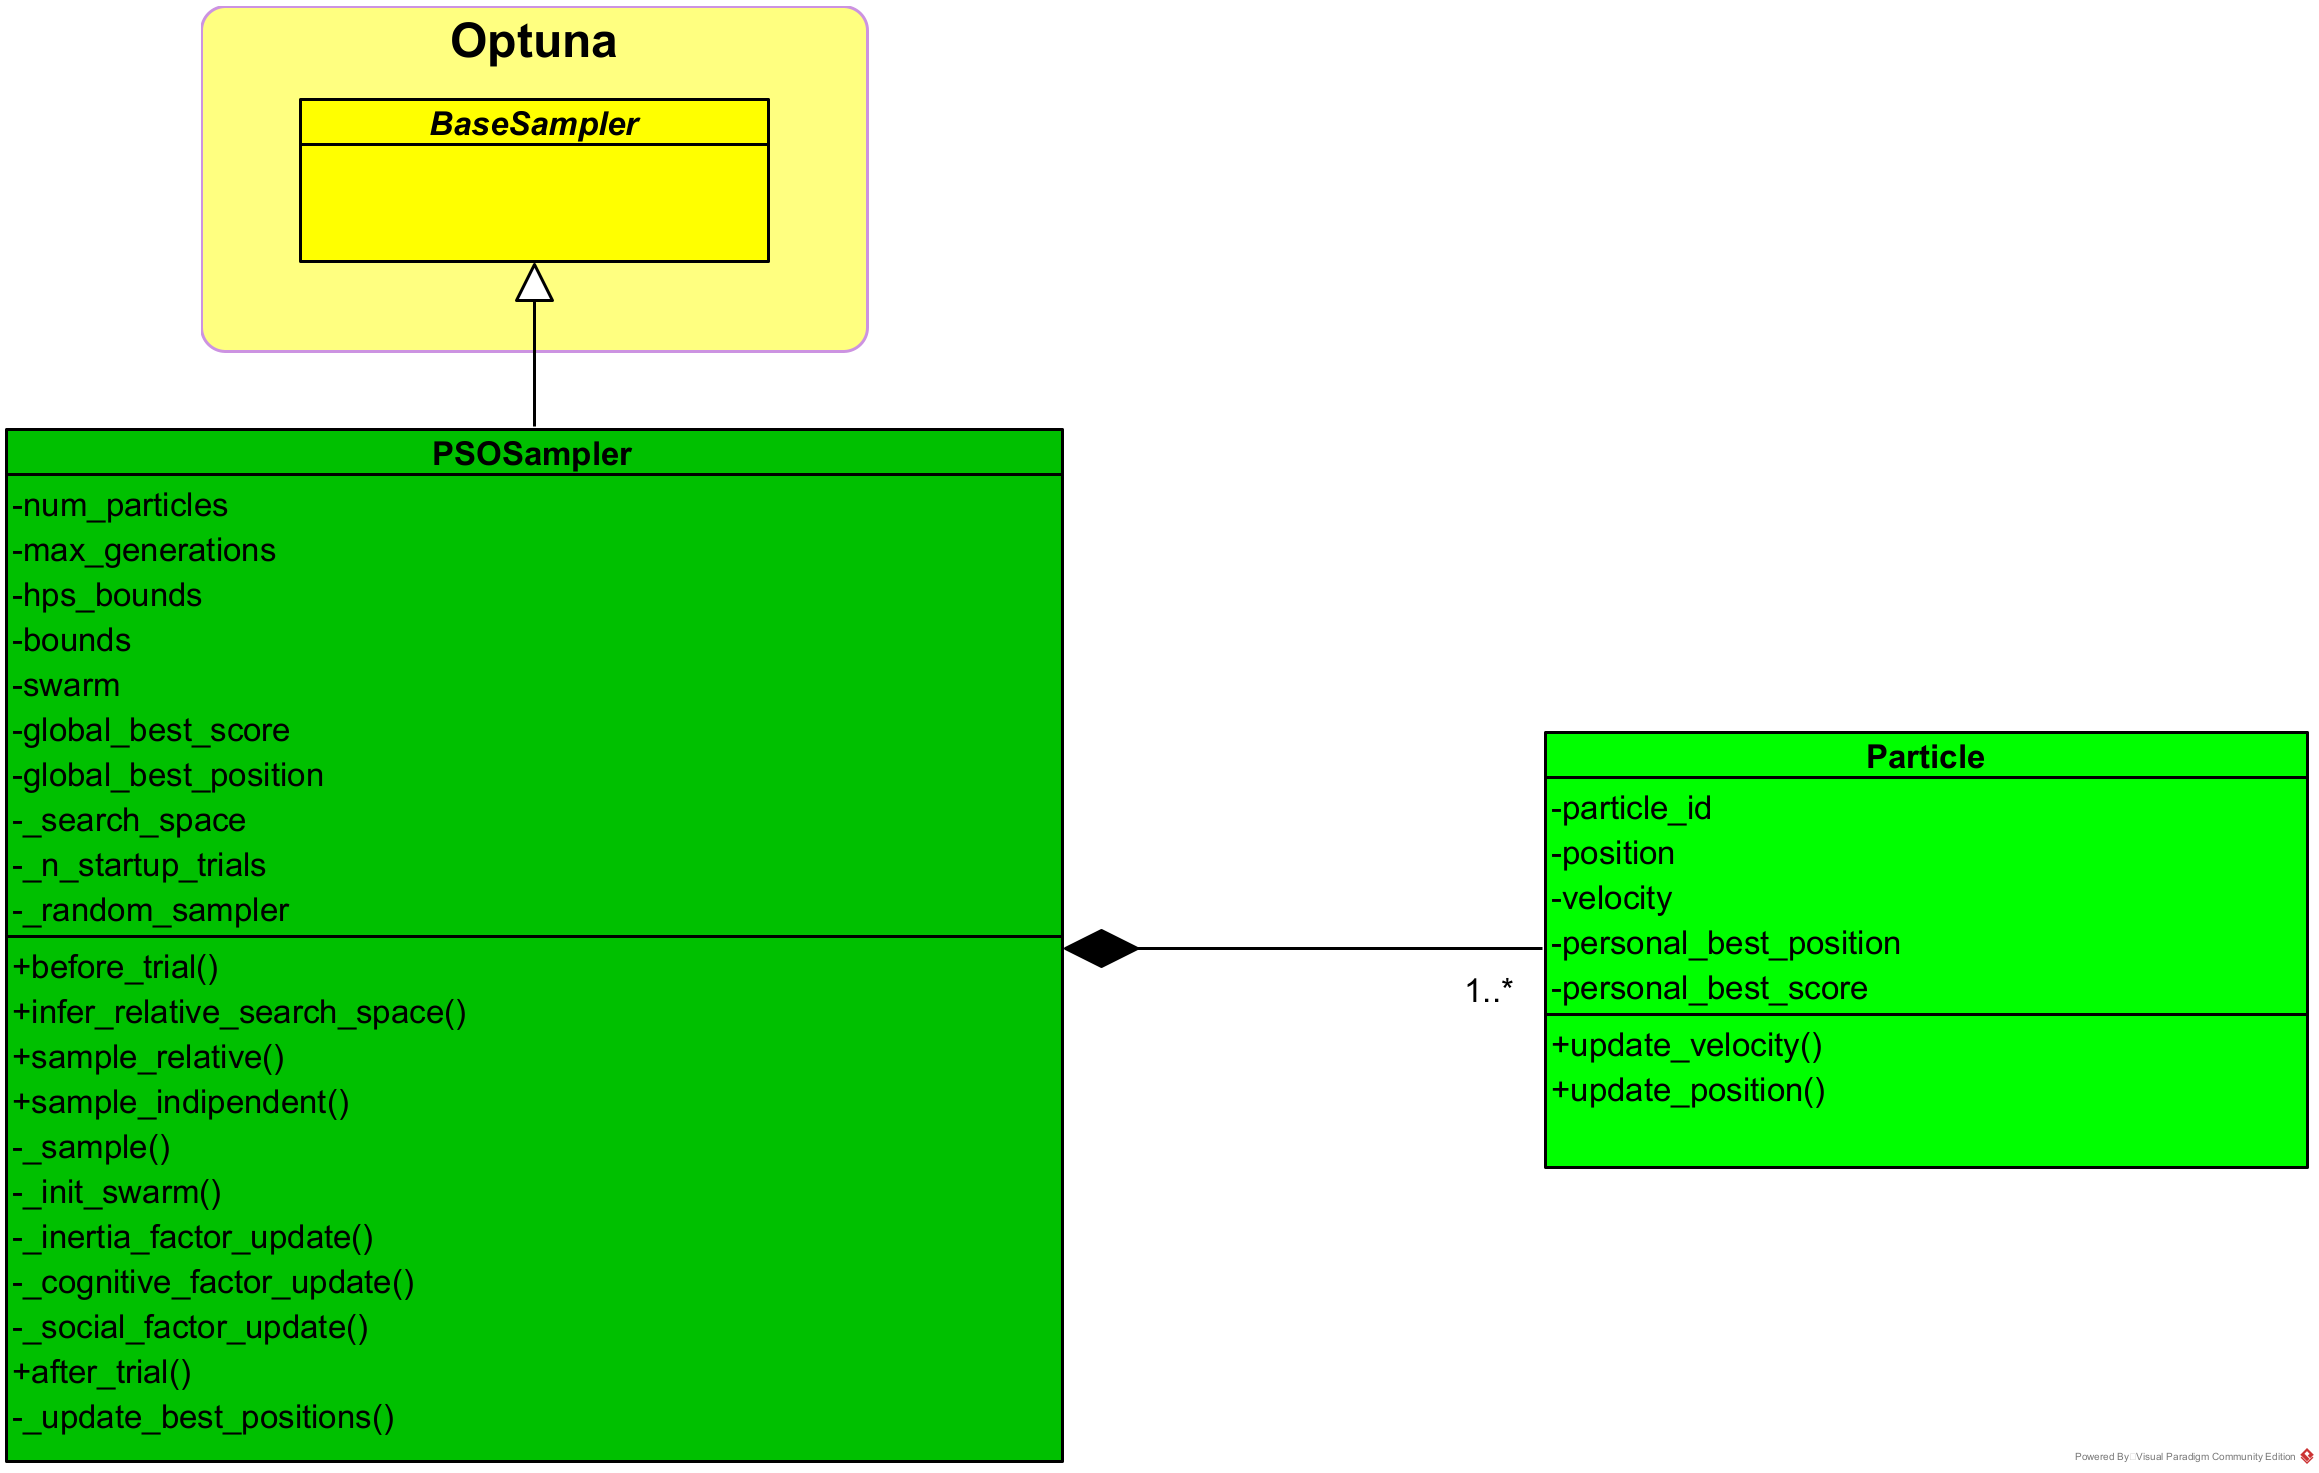
\includegraphics[width=15cm]{figures/figure-3.3.3.png}
% 	\caption[Class Diagram of PSOSampler]{Class Diagram of the implementation of the PSOSampler.}
% 	\label{fig:figure-3.3.3}
% \end{figure}

\subsubsection{Sampling}

At the start of each Trial, the \texttt{before\_trial()} method is called. There, depending on its number, a specific Particle and the current generation are assigned to the Trial.
\\[0.3cm]The Sampling of each candidate tuple of Hyperparameters happens through the \newline\texttt{sample\_relative()} method, which after checking what Particle the current Trial refers to, gets the position of the Particle and converts its coordinates into HPs values.

\subsubsection{After Trial}

At the end of each trial, the \texttt{after\_trial()} method is called.
The Particle associated with the Trial is updated; the values for $w$, $c_1$ and $c_2$ are obtained in the same way described in the section on Custom Implementation of PSO (Sec.~\ref{sec:CustomImplementationOfPSO-3.2}).
Local and Global best positions and scores are also checked and eventually updated.

\section{Applied Neural Network Models}

The type of Machine Learning model chosen for the experiment is Neural Networks.
The chosen library to implement the NN Models and the related support code (such as Loss Function, Train Loop) is PyTorch, which is the most popular Deep Learning library at the moment \cite{PyTorch}.
In the experiments, everything related to the architecture and to the training and evaluation of the models is implemented using PyTorch.

\subsection{Models}

In the experiments, two models have been used: MLP and Lawin.
\\[0.3cm]MLP, or Multi-Layer Perceptron, is the simplest type of Deep Learning Model. The implementation that was utilized is not the standard one of PyTorch but is a custom one, developed using PyTorch. The MLP is applied as the ML model for all the experiments except the last one.
\\[0.3cm]Lawin is a complex DL model specialized in Semantic Segmentation, it is applied only to the Weed Map experiment.

\subsubsection{MLP}

This implementation of the MLP simply follows the standard characteristics of the basic form of MLP (Fig.~\ref{fig:figure-3.4.1}).
Its architecture is represented by a list of values, where the length of the list is the Depth of the Hidden Layer, and the value in the list is the Width of the Layer at the corresponding index.
Both the Architecture and the Activation Function are initialization inputs.
\begin{figure}[t]
	\centering
	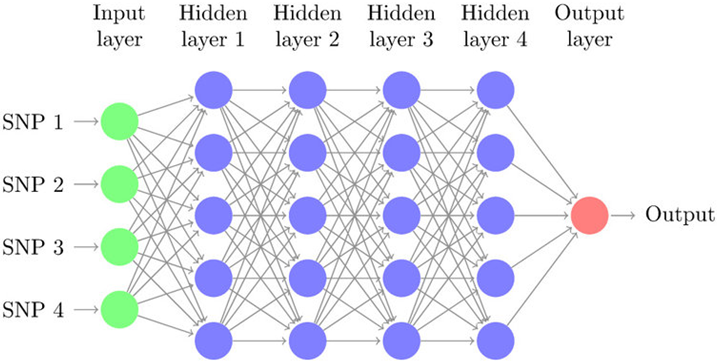
\includegraphics[width=10cm]{figures/figure-3.4.1.png}
	\caption[Visual Example Representation of MLP]{Visual representation of a MLP Neural Network. In this specific example, the input layer consists of four neurons, the output layer of just one, and each hidden layer of five; the width of the hidden part of the network is in this case four. Source: Google Images}
	\label{fig:figure-3.4.1}
\end{figure}
\\[0.3cm]This implementation of MLP refers to the file \texttt{/utils/model/MLP.py} of the code repository \cite{Repository-THESIS}.

\subsubsection{Lawin}\label{sec:Lawin-3.4.1.2}

Lawin is a complex Deep Learning model, in particular is a Vision Transformer, specialized in Semantic Segmentation and applied to Drone Vision problems.
Lawin was developed for this article \cite{WeedMap-PaperThesis}, and its implementation can be found in the relative repository \cite{WeedMap-Repository}.
% 
% \myparagraph{Architecture of Lawin:}
\\[0.3cm]Lawin consists of an Encoder and a Decoder (Fig.~\ref{fig:figure-3.4.2}).
The encoder is a Mix Transformer (MiT), which can generate CNN-like multi-level features with different resolutions, providing a feature map for each Transformer block as output.
The decoder uses a Large Window Attention Spatial Pyramid Pooling (LawinASPP), consisting of five parallel branches, a pooling layer, a shortcut connection, and three large window attentions with different context sizes.
\begin{figure}[t]
	\centering
	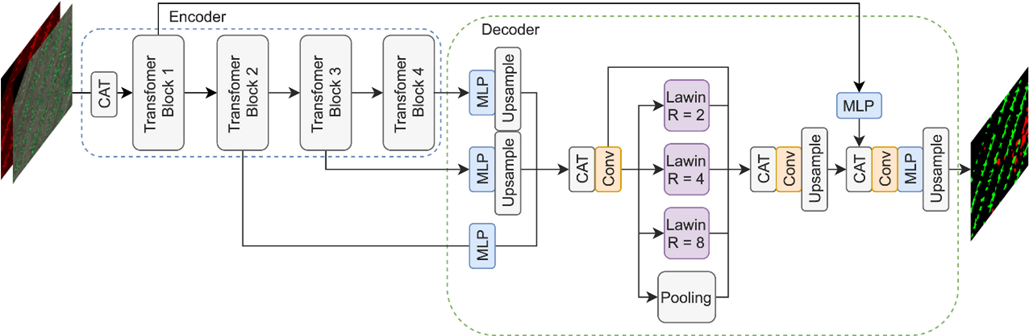
\includegraphics[width=15cm]{figures/figure-3.4.2.png}
	\caption[Architecture of Lawin]{Architecture of Lawin. Source: \cite{WeedMap-PaperThesis}}
	\label{fig:figure-3.4.2}
\end{figure}
% 
% \myparagraph{Variants of Lawin:}
\\[0.3cm]Variants of Lawin are: Double Lawin and Split Lawin.
Those variants are mentioned in this article \cite{WeedMap-PaperThesis} but are not utilized in any of the proposed experiments.

\subsection{Loss Functions}

In Neural Networks, during the training process, the Loss Function calculates the distance between the prediction of the model and the actual target value.
\\[0.3cm]In the experiments, two loss functions have been used, which are Cross Entropy and Focal.
For the Weed Map experiment only FocalLoss has been used, whereas both (or sometimes only CrossEntropyLoss) have been used for all other experiments.
\\[0.3cm]\texttt{CrossEntropy} is the implementation from PyTorch, the one inside the package \texttt{nn}. \texttt{FocalLoss} is implemented with PyTorch.

\subsubsection{Cross Entropy Loss}

Cross Entropy Loss, a loss function principally applied in classification problems, measures the difference between two probability distributions: the true distribution (actual labels) and the predicted distribution (model outputs).
Basically, it determines how far the model's predictions are from the labels (the targets).

\subsubsection{Focal Loss}

Focal Loss is an extension of Cross Entropy Loss. This particular implementation of Focal Loss is from the same article and repository mentioned in the previous sections about Lawin \cite{WeedMap-PaperThesis} \cite{WeedMap-Repository}.
Focal Loss is calculated as follows:
\begin{equation}
	FL=-w_c (1-f(x)_c ) log(f(x)_c)
\end{equation}
In the formula, $f(x)_c$ is the probability of the true class predicted by the model, and $w_c$ is the corresponding class weight.
An interpretation of this formula is that different weights are given to different classes of the classification task. This is to address the class imbalance, particularly in scenarios where some classes are significantly more frequent than others.
\\[0.3cm]A more detailed explanation of Focal Loss is in the earlier mentioned article \cite{WeedMap-PaperThesis}. The original form of Focal Loss was presented in this other article \cite{FocalLoss}.

\subsection{Training and Evaluation}

The functions to train and evaluate the models are also written using PyTorch.
\\[0.3cm]All the code mentioned in this section refers to the package \texttt{/utils/training} of the code repository \cite{Repository-THESIS}. The three illustrated files are \texttt{eval\_step.py}, \texttt{train\_step.py}, and \texttt{train\_loop.py}.

\subsubsection{Training Step}

In the \texttt{train\_step()} function, the PyTorch model is set in Training Mode, and the backward step is executed, calculating the gradients.
Basically, this Training Step is the training loop within a single Epoch.

\subsubsection{Evaluation Step}

In the \texttt{eval\_step()} function the PyTorch model is set in Evaluation Mode, then predictions are made using the validation or test data loaders and compared with the target values.
The performance is evaluated using a specific Metric. In order for this code to be as abstract as possible, a class called \texttt{MetricWrapper} (defined in the \texttt{/utils/metrics} package) was implemented, which abstracts the methods of initialization, computing, and value return of the metrics.
\\[0.3cm]All four main evaluation metrics are calculated (Accuracy, Precision, Recall, F1), but only one is considered toward the final score of the evaluation. The chosen metric is F1 for the Weed Map experiment and Accuracy for all other experiments.

\subsubsection{Training Loop}

In the \texttt{full\_train\_loop()} function, the PyTorch model is fully trained, iterating over the maximum number of epochs, and executing \texttt{train\_step()} and \texttt{eval\_step()} at each iteration.
The function also contains instructions related to pruning, early stopping, logging, and data persistence.

\subsection{Regularization}

Regularization is a technique used to prevent overfitting in Neural Networks. More generally, it is a technique that can be used in multi-objective optimization, to penalize certain characteristics of a candidate solution by lowering its score.
\\[0.3cm]In the proposed experiments, the Regularization technique has the goal of penalizing the complexity of the model, in terms of the width and depth of the hidden layers. Basically, a penalty term is applied referring to the complexity of the model's architecture.
\\[0.3cm]In the experiments, as all of them share a secondary objective to reduce the complexity of the found solutions, a penalization toward architecture complexity was applied. Whenever “Score” is mentioned, it refers to the regularized score, rather than the specific metric score (Accuracy or F1). Which is calculated as follows:
\begin{equation}
	Score = ms - \lambda \cdot complexity
\end{equation}
In the formula: $ms$ is the metric score (could be Accuracy or F1), $\lambda$ (\texttt{lambda}) is the Regularization coefficient (which is passed as input) and $complexity$ is the complexity of the model, which is calculated as the sum of the number of neurons in each hidden layer.
\\[0.3cm]The Regularization was implemented with a \texttt{Regularizer} class defined in the\newline\texttt{/utils/optimization/regularizer.py} file of the code repository \cite{Repository-THESIS}.

\subsection{Other Training-Related Objects}

Inside the \texttt{/utils/model/model\_utils.py} file of the code repository \cite{Repository-THESIS} are defined other aspects of the training process of the model, such as the initialization of Activation Functions and Optimizers.
\\[0.3cm]The possible Activation Functions are Sigmoid, ReLU and Softmax. The \newline\texttt{get\_activation\_fn()} function takes as an input the string sampled from Optuna representing one Activation Function and returns the initialized corresponding object using the PyTorch implementation.
\\[0.3cm]The possible Optimizers are SGD (Stochastic Gradient Descent) and ADAM. The \texttt{get\_optimizer()} function takes as an input the string sampled from Optuna representing one Optimizer and returns the initialized corresponding object using the PyTorch implementation.




\chapter{Results}\label{sec:Chapter4-Results}

In this chapter, the proposed experiments are presented and explained. For each experiment, the results are shown and discussed.
There is a total of five proposed experiments:
\begin{itemize}[itemsep=0.1cm]
    \item \textbf{Experiment 1 - Preliminary Experiment:} aims to demonstrate the necessity of Hyperparameter Optimization (HPO) and to familiarize with the concepts of HPO.
    \item \textbf{Experiment 2 - Comparison of Optuna's Samplers on MNIST:} aims to evaluate the performance of different Hyperparameter Optimization algorithms, specifically Optuna's Samplers, on the MNIST dataset.
    \item \textbf{Experiment 3 - Comparison between a Custom PSO implementation and Optuna:} aims to compare the performance of a custom implementation of Particle Swarm Optimization (PSO) with Optuna's Samplers, on the MNIST dataset.
    \item \textbf{Experiment 4 - Comparison between a PSO Sampler and Optuna's Samplers:} aims to compare the performance of a PSO Sampler (made using Optuna as a base) with the other Optuna's Samplers, on the MNIST dataset.
    \item \textbf{Experiment 5 - Hyperparameter Optimization on Weed Map Dataset:} aims to perform Hyperparameter Optimization on the Weed Map Dataset, using Optuna.
\end{itemize}

\myparagraph{Experiments Source Code:}
All the source code of the experiments is available on the same repository \cite{Repository-THESIS} mentioned in the previous chapter (Chapter~\ref{sec:Chapter3-Methodology}), specifically in the \texttt{/experiments/} package.
In particular, the Weed Map Experiment (Experiment 5) is in the file \newline\texttt{/weed\_mapping\_experiment/Weed\_Mapping\_Optimization.ipynb}, while the other experiments were run using \texttt{/MNIST\_experiment/MNIST\_Optimization.ipynb}.

\section{Experiment 1 - Preliminary Experiment}

This Preliminary Experiment has a double goal.
The first is to familiarize with the concepts of HPO from a physical implementation perspective.
The second reason is to establish, if ever needed, the necessity of Hyperparameter Optimization; to demonstrate that HPO can actually improve the final performance of a ML experiment by finding the best Hyperparameters to train the model subject of the experiment with.
\\[0.3cm]Note that in this preliminary experiment, everything was developed with simple vanilla Python, without the use of the infrastructure described in the previous chapter (Chapter~\ref{sec:Chapter3-Methodology}).

\myparagraph{System used for the Experiment:}
The hardware that was utilized to run this experiment is the following:
\begin{itemize}[itemsep=0.1cm]
    \item CPU: Intel Core i5-8265U CPU @ 1.60GHz (4-core, 8 thread)
    \item GPU: NVIDIA GeForce MX 110 (2GB VRAM)
    \item RAM: 8GB (DDR4)
    \item Disk: SSD
    \item OS: Windows 11
\end{itemize}

\subsection{Preparation of the Experiment}

Given the first goal of the experiment, the idea is to realize a simple implementation of the most traditional of HPO algorithms, which is Grid Search.
\\[0.3cm]The first part of the experiment consists in recreating another ML experiment which does not apply HPO and evaluating its results. Successively, the hyperparameters of that same ML model will be optimized with the custom Grid Search.
\\[0.3cm]The experiment chosen for comparison is the one proposed by the book “Dive Into Deep Learning” \cite{Tesi-1.6} (chapter 4 of the book). Some modifications have been made to this experiment: a simpler version of the proposed dataset is used; the Multi-Layer Perceptron (MLP) considered is implemented with vanilla Python rather than PyTorch.

\subsubsection{Dataset of the Experiment:}
The Dataset considered for the experiment is a simplified version of MNIST, specifically, the version included in scikit-learn \cite{scikit-learn}, from the function \texttt{load\_digits()} of the \texttt{dataset} module. (An explanation of the complete MNIST dataset is in the next experiment; for this preliminary experiment it is not necessary to understand the dataset).

\subsubsection{Model and Hyperparameters of the Experiment:}
As introduced earlier, the MLP model utilized is not the same as the one from the book. This is not detrimental to the scientific value of the experiment, as the considered hyperparameters and configuration of the model were the same as those proposed in the book, so that a comparison would still be possible.

\subsubsection{Implementation of Grid Search:}
The proposed implementation of Grid Search is completely made from scratch.
The algorithm takes as input the model, the dataset, and the grid of hyperparameters; the grid is a map object, where the keys are strings that represent the name of the hyperparameter, and the values are lists which contain the values that the corresponding hyperparameter can be.
\\[0.3cm]At the start of the algorithm, a Cartesian Product is applied to the lists inside the \texttt{param\_grid}, basically generating all the trials that are going to be evaluated.
For each trial, the model is initialized with the hyperparameters of that trial and evaluated; the results are saved in a variable.
After having completed all the trials, the algorithm returns as output the variable containing all the results, from which the best trial can be obtained.
\\[0.3cm]Two versions of this algorithm have been developed, one without parallelism and one with parallelism. There is no difference between the two, the only one is that the second allows to execute multiple trials on multiple threads.

\subsection{Execution of the Experiment}

The execution of the experiment is divided into three short parts: run and evaluation without hyperparameter optimization; run and evaluation with hyperparameter optimization; comparison of results.
\\[0.3cm]The set of hyperparameter utilized by the book for the experiment are the following (Tab.~\ref{tab:table-4.1.1}).
\begin{table}[ht!]
	\center
	\setlength{\tabcolsep}{0.5cm}
	\caption[Initial Hyperparameters of Experiment 1]{Initial hyperparameters of Experiment 1, as proposed by the book.}
	\begin{tabular}{@{}lc@{}}
		\toprule
		\textbf{Hyperparamter} & \textbf{Value} \\ \midrule
		Activation Input       & Sigmoid               \\[0.1cm]
		Activation Output      & Softmax               \\[0.1cm]
		Batch Size             & 256                   \\[0.1cm]
		Learning Rate          & 0.1                   \\[0.1cm]
		Hidden Size            & 10                    \\[0.1cm]
		Epochs                 & 10000                 \\ \bottomrule
	\end{tabular}
	\label{tab:table-4.1.1}
\end{table}
Training and evaluating the model with these hyperparameters lead to results of 99\% accuracy on the Training Set and 97\% on the Test Set.
The custom Grid Search algorithm is executed with the \texttt{param\_grid} in the figure (Fig.~\ref{fig:figure-4.1.1}) as input.
\begin{figure}[t]
	\centering
	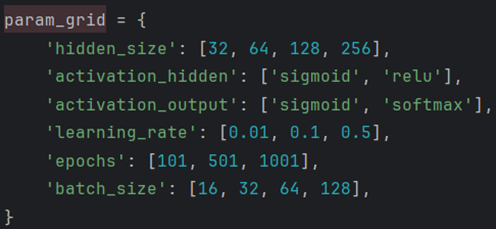
\includegraphics[width=8cm]{figures/figure-4.1.1.png}
	\caption[Param Grid for Custom Grid Search Experiment]{The Param Grid utilized for the Custom Grid Search Experiment.}
	\label{fig:figure-4.1.1}
\end{figure}
\\[0.3cm]The Grid Search algorithm executed a total of 576 trials. After the completion of the Optimization, there are three best results (with the same accuracy), which are in the figure (Fig.~\ref{fig:figure-4.1.2}).
\begin{figure}[b]
	\centering
	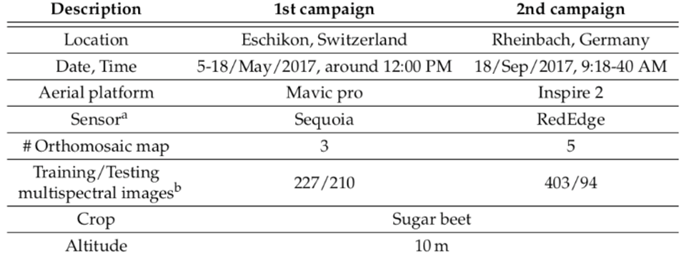
\includegraphics[width=15cm]{figures/figure-4.1.2.png}
	\caption[Best Results of Custom Grid Search Experiment]{The three best results of the Custom Grid Search Experiment.}
	\label{fig:figure-4.1.2}
\end{figure}
\\[0.3cm]These best results have an accuracy of 100\% on the Training Set and 98.6\% on the Test Set. Moreover, there are more than 20 trials with better accuracy than the configuration proposed by the book.

\subsection{Discussion of the Results}

This simple experiment with its results outlines how hyperparameter optimization, even when using a simple implementation of the weakest algorithm, could lead to a significant improvement in the performance of the trained model.
\\[0.3cm]The gained 1.6\% accuracy on the Test Set may seem like a little improvement, but is remarkable, especially when the dataset is composed of a very large number of observations.
\\[0.3cm]These results, additionally, confirm another aspect of HPO, which is the ability to improve the performance of an experiment without interfering with the model or the dataset.

\section[Experiment 2 - Comparison of Optuna's Samplers]{Experiment 2 - Comparison of Optuna's Samplers on MNIST}\label{sec:Experiment2-4.2}

The objective of this experiment is to evaluate the performance of different Hyperparameter Optimization algorithms so as to gain general knowledge about the capacity of each in preparation for subsequent, more complex experiments.
\\[0.3cm]In order to make the results and the methodology as much scientifically comparable as possible, rather than implementing various Samplers from scratch individually, a library for HPO is used.
\\[0.3cm]The chosen library is Optuna, which, as described in previous sections, includes a few Samplers already implemented, with the same style and same preconditions, making each optimization perfectly comparable to one another.
\\[0.3cm]As the idea is to have results that are as much general as possible, and because such “optimization of optimizations” is inevitably enormously expensive, a simple dataset is considered, which is MNIST.

\myparagraph{System used for the Experiment:}
The hardware that was utilized to run this experiment is the following:
\begin{itemize}[itemsep=0.1cm]
	\item CPU: Intel Core i7-10700K CPU @ 3.80GHz
	\item GPU: NVIDIA GeForce RTX 3080 (10GB VRAM)
	\item RAM: 16GB (DDR5)
	\item Disk: SSD
	\item OS: Linux (Ubuntu)
\end{itemize}

\subsection{MNIST Dataset}

The MNIST Dataset is a database of images of handwritten digits \cite{MNIST}.
MNIST is the ideal dataset for learners and for small experiments regarding the field of pattern recognition, is basically a benchmarking dataset for Image Classification.
\\[0.3cm]Each image of the MNIST Dataset represents a digit from 0 to 9, making it ideal for benchmarking simple classification models for images (Fig.~\ref{fig:figure-4.1.3}).
\begin{figure}[t]
	\centering
	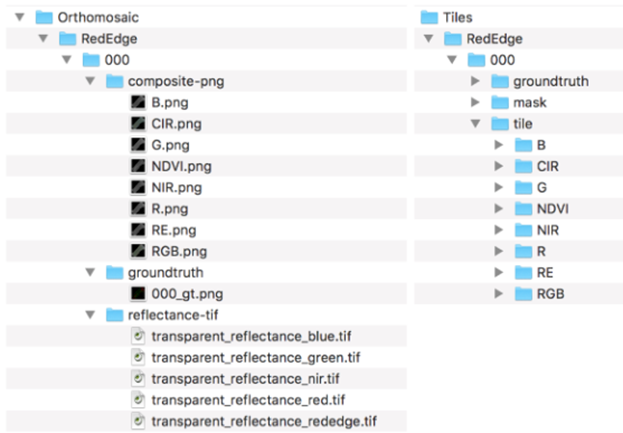
\includegraphics[width=9cm]{figures/figure-4.1.3.png}
	\caption[Examples of MNIST Images]{Some examples of images in the original MNIST dataset. Source:~\cite{MNIST}}
	\label{fig:figure-4.1.3}
\end{figure}

\subsubsection{Structure of MNIST Dataset}

The MNIST Dataset is composed of a total of 70000 images, of which 60000 are part of the training set and 10000 are part of the test set \cite{MNIST}.
The total weight of MNIST is 11.6MB when compressed, 52.3MB normally. Each image is 28x28 pixels, is in black and white, and weighs 784 bytes.

\myparagraph{NIST Dataset:}
MNIST is a newer version of an old dataset called NIST, in which the division was between SD-1 (Special Database 1) and SD-3 (Special Database 3); where SD-3 was the training set, and SD-1 the test set. The images of SD-3 were much clearer and easier to recognize.
\\[0.3cm]MNIST is designed so that half of its training images and half of its test images come from SD-1 and the remaining half from SD-3.
This means that half of the images of MNIST are easier to recognize, the other half are more difficult.

\subsubsection{Variants of MNIST Dataset}
Given its extreme simplicity to both use and understand, MNIST has inspired numerous variants. Some of the most famous variants are the following:
\begin{itemize}[itemsep=0.1cm]
    \item \textbf{Fashion-MNIST:} replaces digits with images of clothing items to test models on more complex visual patterns (Fig.~\ref{fig:figure-4.1.4}).
    \begin{figure}[t]
		\centering
		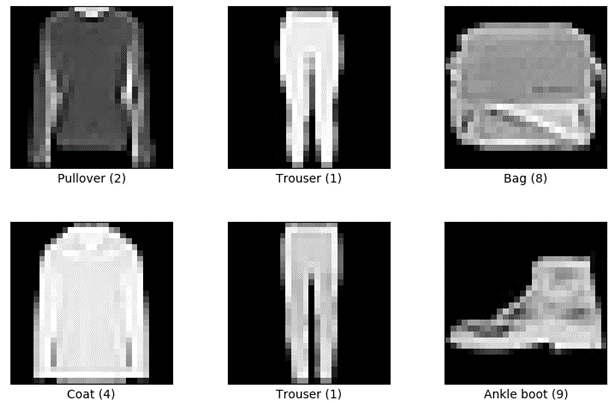
\includegraphics[width=10cm]{figures/figure-4.1.4.png}
		\caption[Examples of Fashion-MNIST Images]{Some examples of images in the Fashion-MNIST dataset. Source: Google Images}
		\label{fig:figure-4.1.4}
	\end{figure}
	\item \textbf{EMNIST (Extended MNIST):} includes, in addition to digits, also letters, to enhance the diversity of the dataset.
    \item \textbf{KMNIST:} includes images of Japanese Kanji characters, making the classification task much more complex than the version on the Latin alphabet.
    \item \textbf{NoiseMNIST:} is a version of MNIST where Gaussian noise is added to the images, it is useful to test the robustness of the model against noisy data.
    \item \textbf{Rotated MNIST:} is a version of MNIST where the images are rotated by a random angle, to test the robustness of the model against rotated data.
\end{itemize}
% 
% \myparagraph{Fashion-MNIST:}
% Fashion-MNIST replaces digits with images of clothing items to test models on more complex visual patterns.
% \begin{figure}[t]
% 	\centering
% 	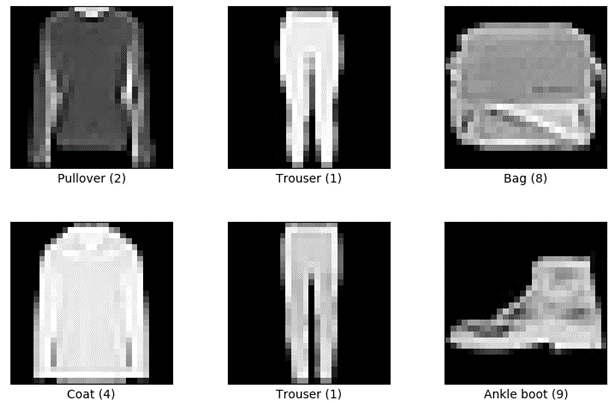
\includegraphics[width=15cm]{figures/figure-4.1.4.png}
% 	\caption[Examples of Fashion-MNIST Images]{Some examples of images in the Fashion-MNIST dataset. Source: Google Images}
% 	\label{fig:figure-4.1.4}
% \end{figure}
% 
% \myparagraph{EMNIST (Extended MNIST):}
% EMNIST includes, in addition to digits, also letters, to enhance the diversity of the dataset.
% 
% \myparagraph{KMNIST:}
% KMNIST includes images of Japanese Kanji characters, making the classification task much more complex than the version on the Latin alphabet.
% 
% \myparagraph{NoiseMNIST:}
% NoiseMNIST is a version on MNIST where Gaussian noise is added to the images, it is useful to test the robustness of the model against noisy data.

\subsection{Preparation of the Experiment}

The preparation for the experiment is simple: using the code infrastructure described in the Methodology chapter, specifically the section on Optuna Enhancing (Sec.~\ref{sec:EnhancingOptuna-3.3}), an Optuna's \texttt{Study} object is created and run.
\\[0.3cm]The MNIST dataset was imported through the \texttt{MNIST} package of Pytorch, included in torchvision, and then loaded with PyTorch data loaders.

\subsubsection{Setup of the Studies}

% \myparagraph{Initialize the Studies:}
The Samplers of Optuna subject of this experiment are the following: \texttt{RandomSampler}, \texttt{TPESampler}, \texttt{CmaEsSampler}, \texttt{GPSampler}, \texttt{NSGAIISampler}, \texttt{PartiallyFixedSampler}, \texttt{QMCSampler}.
For each of the Samplers, an Optuna \texttt{Study} is created. All the samplers are initialized with their default input values.
\\[0.3cm]The Pruner utilized for each Study is the Hyperband (\texttt{HyperbandPruner} object in Optuna), initialized with its default input values.

\subsubsection{Setup of the Objective Function}

% \myparagraph{Objective Function:}
The objective function, obviously the same for each Study, is divided into three sections: Declaration of the Hyperparameters to optimize and their value ranges; Initialization of the model and related objects; Training and Evaluation of the model.
\\[0.3cm]At the execution of each trial, for each hyperparameter, a value is sampled by Optuna's Sampler, then those values are used to initialize the model and its related objects, training included, and the training loop can start. The value then returned will be the score.
% 
% \myparagraph{Search Space of Hyperparameters:}
\\[0.3cm]The Hyperparameters declared in the objective function, which form the Search Space of the Study, for this experiment were the following (Tab.~\ref{tab:table-4.2.1}).
\begin{table}[ht!]
	\center
	\setlength{\tabcolsep}{0.5cm}
	\caption[Search Space of Experiment 2]{Search Space of Experiment 2: list of hyperparameters and their values ranges, with the step. Where Step is $\sim$ if the range is continuous.}
	\begin{tabular}{@{}lcc@{}}
		\toprule
		\textbf{Hyperparamter}   & \textbf{Range}             & \textbf{Step} \\ \midrule
		Activation Function      & \{ReLU, tanh, sigmoid\}    & -             \\[0.1cm]
		Batch Size               & {[}16, 64{]}               & 16            \\[0.1cm]
		Epochs                   & 10                         & -             \\[0.1cm]
		Hidden Layer Width \{i\} & {[}8, 128{]}               & 8             \\[0.1cm]
		Hidden Layer Depth       & {[}1, 3{]}                 & 1             \\[0.1cm]
		Learning Rate            & {[}$10^{-5}$, $10^{-1}${]} & $\sim$        \\[0.1cm]
		Loss Function            & \{CrossEntropy, Focal\}    & -             \\[0.1cm]
		Optimizer                & \{SGD, Adam\}              & -             \\ \bottomrule
	\end{tabular}
	\label{tab:table-4.2.1}
\end{table}
% 
% \myparagraph{Optimizing Process Parameters:}
\\[0.3cm]Other parameters, related to the Optimization process, basically hyperparameters of the HPO process itself (could be called “Hyper-Hyperparamters”), which were used are the following (Tab.~\ref{tab:table-4.2.2}).
\begin{table}[ht!]
	\center
	\setlength{\tabcolsep}{0.5cm}
	\caption[Optimization External Parameters of Experiment 2]{External optimization parameters of Experiment 2, basically hyperparameters of the optimization process, with their values.}
	\begin{tabular}{@{}llc@{}}
		\toprule
		\textbf{Group} & \textbf{Parameter} & \textbf{Value} \\ \midrule
		Regularizer    & labda              & 0.4            \\[0.1cm]
		EarlyStopper   & patience           & 5              \\ \bottomrule
	\end{tabular}
	\label{tab:table-4.2.2}
\end{table}

\subsection{Execution of the Experiment}

The execution of each Study is handled by an \texttt{OptunaRunner} object, which at the end of the optimization process saves the results on a csv file.
\\[0.3cm]The number of Trials executed for each Study was 128.
\\[0.3cm]In the reporting of the results, the information regarding what the best hyperparameters' values are will be ignored, because it is not the focus of the experiment, which is to identify how well performing the various techniques are.
\\[0.3cm]For the experiment, each Study has been executed around six times (some had more executions than others); the reported results are therefore a mean of the multiple results from the multiple executions. 

\subsubsection{RandomSampler}

The best score achieved by the \texttt{RandomSampler} is 91.7\%; there are 29 trials with a score over 80\% and 3 with a score over 90\%. The Accuracy of these top trials is around 95\%-97\%.
\\[0.3cm]In terms of Accuracy, the best score is 98\% and the best results are around 97\%, but those results have lower regularized scores.
\\[0.3cm]The results of the \texttt{RandomSampler} are useful to compare the results of the other samplers, to see if there is an actual advantage in using them for these experiments, or if they are just equivalent to the random approach.

\subsubsection{TPESampler}

The best score achieved by the \texttt{TPESampler} is 94\%, which is the best score of the whole experiment; there are 101 trials with a score over 80\%; 60 with a score over 90\%; 13 with a score over 93\%. The Accuracy of these top trials is around 94\%-96\%.
\\[0.3cm]In terms of Accuracy, the best scores are all close to 98\%, but all those best scores are also the worst in terms of regularized score.
\\[0.3cm]Talking about the network architectures, the best scores were achieved with a single hidden layer architecture, other good scores were achieved even with a linear architecture, or with a two-hidden-layer architecture where the total number of neurons was minimally higher than the single layer one.

\subsubsection{CmaEsSampler}

After a total of five tries, the execution of the studies never terminated without errors.
It is likely that the setup values of the experiment are not compatible with the default initialization values of this sampler.
Therefore, this Sampler will be discarded.

\subsubsection{GPSampler}

The best scores achieved by \texttt{GPSampler}, both in terms of Accuracy and in terms of regularized score, are basically equivalent to the results of \texttt{RandomSampler}.
In order to give more possibilities to the sampler, various initialization values were tried, none of which changed the results.
It is not completely clear why this sampler produces results equivalent to those of \texttt{RandomSampler}, this will be further discussed in the Discussion section.

\subsubsection{NSGAIISampler}

The best scores achieved by \texttt{NSGAIISampler}, both in terms of Accuracy and in terms of regularized score, are basically equivalent to the results of \texttt{RandomSampler}.
In order to give more possibilities to the sampler, various initialization values were tried, none of which changed the results.
It is not completely clear why this sampler produces results equivalent to those of \texttt{RandomSampler}, this will be further discussed in the Discussion section.

\subsubsection{PartiallyFixedSampler}

The \texttt{PartiallyFixedSampler} was failing in the first execution because, as the name suggests, it is a type of sampler that requires some hyperparameters of the defined Search Space to be fixed.
\\[0.3cm]The choice was not to further continue using this sampler, as the objective of the experiment is to evaluate the sampling technique rather than to actually find the best hyperparameters' values, or correlations in the Search Space.
Therefore, this Sampler will be discarded.

\subsubsection{QMCSampler}

The best scores achieved by \texttt{QMCSampler}, both in terms of Accuracy and in terms of regularized score, are basically equivalent to the results of \texttt{RandomSampler}.
In order to give more possibilities to the sampler, various initialization values were tried, none of which changed the results.
It is not completely clear why this sampler produces results equivalent to those of \texttt{RandomSampler}, this will be further discussed in the Discussion section.

\subsection{Discussion of the Results}

This experiment, with the execution of these studies, allowed to establish important ground knowledge about the efficacy of the most important sampling techniques of Hyperparameter Optimization.

\subsubsection{Analysis of the Best Hyperparameters Results}

For the record, even if it is not in the main objectives of the experiment, the best hyperparameters found by the most reliable Sampler (\texttt{TPESampler}) were the following (Tab.~\ref{tab:table-4.2.3}).
% \begin{itemize}[itemsep=0.1cm]
%     \item Activation = ReLU
%     \item Loss = CrossEntropy
%     \item Architecture = [input, 16, output]
%     \item Batch Size = 16
%     \item Optimizer = Adam
% \end{itemize}
\begin{table}[ht!]
	\center
	\setlength{\tabcolsep}{0.5cm}
	\caption[Best Hyperparameters of Experiment 2]{Best hyperparameters of Experiment 2, found by with the optimization process with \texttt{TPESampler}.}
	\begin{tabular}{@{}lc@{}}
		\toprule
		\textbf{Hyperparamter} & \textbf{Value}          \\ \midrule
		Activation             & ReLU                    \\[0.1cm]
		Loss                   & CrossEntropy            \\[0.1cm]
		Architecture           & {[}input, 16, output{]} \\[0.1cm]
		Batch Size             & 16                      \\[0.1cm]
		Optimizer              & Adam                    \\ \bottomrule
	\end{tabular}
	\label{tab:table-4.2.3}
\end{table}
It is vital to note that, given the simplicity of the dataset, in some executions, the best hyperparameters' values were different (except model architecture), outlining how in simple problems like this one, the only really impactful factor was the architecture of the NN, while the possible combinations of the other hyperparameters able to achieve high results were many.

\subsubsection{Analysis of the Failed Samplers}

With regard to the two failed sub-experiments, which are, the studies using respectively \texttt{CmaEsSampler} and \texttt{PartiallyFixedSampler}, for the sake of simplicity, these samplers will be discarded.
In order to conduct the next experiments, it was already necessary to identify the best samplers and discard the worst ones; so, discarding the failing samplers is the least time-consuming solution.

\subsubsection{Analysis of the Worst Performing Samplers}

As for the performance of \texttt{GPSampler}, \texttt{NSGAIISampler} and \texttt{QMCSampler}, one possible hypothesis for the reason their results are equivalent to \texttt{RandomSampler}, is the simplicity of the dataset and the model.
\\[0.3cm]The hypothesis is, given that, as mentioned above, there is only one impactful hyperparameter, it is unlikely for these more complex sampling algorithms to find correlations in the Search Space, making the search partially unsuccessful.
Therefore, for the next experiments, these three samplers will be discarded.

\subsubsection{Analysis of the Best Samplers}

The best results were obtained by the Study using \texttt{TPESampler}. The trend in the results suggests that the \texttt{TPESampler} is actually learning from past trials throughout the optimization process, as the best results are mostly in the later stages of the optimization.
\\[0.3cm]Therefore, with regard to the first objective of the experiment, it can be concluded that \texttt{TPESampler} can be used for the other experiments. Together with \texttt{TPESampler}, also \texttt{RandomSampler} can be used, because it did not show any unexpected behaviour and can thus be applied to make first assessments.
\\[0.3cm]In conclusion, now that the best performing samplers are well-established, in the next experiments they can be utilized as a tool of comparison with other new sampling techniques. 

\subsubsection{Analysis of the Best NN Architectures}

For what concerns the second objective of the experiment, which is to find lightweight, but well-performing nonetheless solutions, \texttt{TPESampler} gained interesting results.
\\[0.3cm]The theoretical hypothesis was that, at the same total number of neurons, deeper architectures would have reached better scores. The results suggest, however, that there is no difference between the two, sometimes even linear architectures have achieved a good score.
\\[0.3cm]From these results, it can be concluded that the experiment, and especially the model, are too simple for the score to be significantly different between deeper and less deep networks. Deeper networks do not result in an increase in generalization power if the model and the experiment are excessively simple.

\section[Experiment 3 - Comparison: Custom PSO vs Optuna]{Experiment 3 - Comparison between a Custom PSO implementation and Optuna}

The goal of this experiment is to test and evaluate the functioning and performance of the custom implementation of Particle Swarm Optimization, adapted for HPO in a way that is similar to Optuna, and compare such performance to that of the samplers of Optuna.
\\[0.3cm]In order to make the results and the methodology as much scientifically comparable as possible, as described in the methodology chapter (Sec.~\ref{sec:CustomImplementationOfPSO-3.2}), the implementation of PSO replicates almost perfectly the functioning of Optuna and displays the result in the same exact way.
\\[0.3cm]As the goal of the experiment is primarily to compare a new technique to existent techniques, and therefore would be excessive to operate on a complex and expensive problem, a simple dataset is considered, which again is MNIST.

\myparagraph{System used for the Experiment:}
The hardware that was utilized to run this experiment is the same as Experiment 2 (Sec.~\ref{sec:Experiment2-4.2}).

\subsection{Preparation of the Experiment}

The preparation for the experiment is similar to Experiment 2 (Sec.~\ref{sec:Experiment2-4.2}): the Studies related to the samplers of Optuna continue to be initialized with the “wrapping”, whereas the Study for the custom PSO is initialized separately. Nevertheless, the process is basically the same, given that it is supposed to be a sort of replica of Optuna. 
\\[0.3cm]The MNIST dataset was imported through the \texttt{MNIST} package of Pytorch, included in torchvision, and then loaded with PyTorch data loaders.

\subsubsection{Setup of the Studies}

% \myparagraph{Initialize the Studies:}
The Samplers of Optuna subject of this experiment are the following: \texttt{RandomSampler}, \texttt{TPESampler}.
For each of the Samplers, an Optuna \texttt{Study} is created. All the samplers are initialized with their default input values.
The Study of the custom PSO is called \texttt{PSO\_optimization}.
\\[0.3cm]As a result of the subsequent lack of scientific comparability between the two approaches if the pruning mechanism was involved for both, the Pruner is disabled.

\subsubsection{Setup of the Objective Function}

% \myparagraph{Objective Function:}
The objective function is the same for each Study, even for the \texttt{PSO\_optimization} Study. The structure of the objective function is the same as the last experiment.
% 
% \myparagraph{Search Space of Hyperparameters:}
\\[0.3cm]The Hyperparameters declared in the objective function, which form the Search Space of the Study, for this experiment were the following (Tab.~\ref{tab:table-4.3.1}).
\begin{table}[ht!]
	\center
	\setlength{\tabcolsep}{0.5cm}
	\caption[Search Space of Experiment 3]{Search Space of Experiment 3: list of hyperparameters and their values ranges, with the step. Where Step is $\sim$ if the range is continuous.}
	\begin{tabular}{@{}lcc@{}}
		\toprule
		\textbf{Hyperparamter} & \textbf{Range}             & \textbf{Step} \\ \midrule
		Activation Function    & \{ReLU, tanh, sigmoid\}    & -             \\[0.1cm]
		Hidden Layer Width 1   & {[}0, 128{]}               & 1             \\[0.1cm]
		Hidden Layer Width 2   & {[}0, 128{]}               & 1             \\[0.1cm]
		Hidden Layer Width 3   & {[}0, 128{]}               & 1             \\[0.1cm]
		Learning Rate          & {[}$10^{-4}$, $10^{-2}${]} & $\sim$        \\[0.1cm]
		Optimizer              & \{SGD, Adam\}              & -             \\ \bottomrule
	\end{tabular}
	\label{tab:table-4.3.1}
\end{table}
% 
% \myparagraph{Optimizing Process Parameters:}
\\[0.3cm]Other parameters, related to the Optimization process, basically hyperparameters of the HPO process itself (could be called “Hyper-Hyperparamters”), which were used are the following (Tab.~\ref{tab:table-4.3.2}).
\begin{table}[ht!]
	\center
	\setlength{\tabcolsep}{0.5cm}
	\caption[Optimization External Parameters of Experiment 3]{External optimization parameters of Experiment 3, basically hyperparameters of the optimization process, with their values.}
	\begin{tabular}{@{}llc@{}}
		\toprule
		\textbf{Group}               & \textbf{Parameter} & \textbf{Value} \\ \midrule
		Regularizer                  & labda              & 0.4            \\[0.1cm]
		EarlyStopper                 & patience           & 5              \\[0.2cm]
		\multirow{2}{*}{PSOStopping} & patience           & 5              \\[0.1cm]
									 & tolerance          & 0.005          \\[0.2cm]
		\multirow{2}{*}{PSO}         & num\_particles     & 32             \\[0.1cm]
									 & max\_generations   & 8              \\ \bottomrule
	\end{tabular}
	\label{tab:table-4.3.2}
\end{table}

\subsection{Execution of the Experiment}

The execution of each Study is handled by an \texttt{OptunaRunner} object for Optuna and by \texttt{PSORunner} for PSO (it is exactly the same); which, at the end of the optimization process, saves the results on a csv file.
\\[0.3cm]The number of Trials executed for each Study was 256.
\\[0.3cm]In the reporting of the results, the information regarding what the best hyperparameters' values are will be ignored, because it is not the focus of the experiment, which is to identify how well performing the various techniques are.

\subsubsection{RandomSampler}

The best score achieved by the \texttt{RandomSampler} is 92\%; there are 42 trials with a score over 80\% and 2 with a score over 90\%. The Accuracy of these top trials is around 95\%-97\%.
\\[0.3cm]In terms of Accuracy, the best score is 98\% and the best results are around 97\%, but these results have far lower regularized scores.
\\[0.3cm]As every experiment, these results from the \texttt{RandomSampler} have the purpose of evaluating how well the new techniques are performing, and whether they are doing what supposed to or are just collapsing into a random sampling.

\subsubsection{TPESampler}

The best score achieved by the \texttt{TPESampler} is 93.2\%, there are 224 trials with a score over 80\%; 135 with a score over 90\%; 5 with a score over 93\%. The Accuracy of these top trials is around 95\%-96\%.
\\[0.3cm]In terms of Accuracy, the best scores are all around 97\%, but these results have far lower regularized scores.

\subsubsection{PSO\_optimization}

The best score achieved by the custom PSO algorithm is 93\%, there are 123 trials with a score over 80\%; 22 with a score over 90\%; 2 with a score over 93\%. The Accuracy of these top trials is around 95\%-96\%.
\\[0.3cm]In terms of Accuracy, the best scores are all close to 98\%, but these results have far lower regularized scores.

\subsection{Discussion of the Results}

The results of the experiment allow to safely conclude that the proposed adaptation of PSO to HPO was successful and is also perfectly comparable with the results from the Studies of Optuna.

\subsubsection{Analysis on the Custom PSO Results}

The results presented by the \texttt{PSO\_optimization} Study, allow to establish that the algorithm is working as intended, the process is learning from past Trials.
Analysing the results, it appears evident that the best scores have been obtained at the latest generations, outlining how the Particles are correctly closing their distance with the global optimum over time.

\subsubsection{Analysis of the Comparison with Optuna}

After comparing the results from the \texttt{PSO\_optimization} Study, \texttt{RandomSampler} and \texttt{TPESampler}, it is easy to see that the PSO reaches similar levels of quality.
\\[0.3cm]The comparison with \texttt{RandomSampler} clearly shows that the PSO is not sampling randomly, but is following a logic, based on the PSO algorithm.
\\[0.3cm]The comparison with \texttt{TPESampler} allows to say that PSO is also extremely well-performing, and can be used in the same way as the TPESampler. The former has indeed found a greater number of very good solutions, but this is also because PSO has the tendency to never stop the exploration; in fact, watching the trial number around which the two algorithms started to find good solutions, it is almost the same; the main difference is a result of the characteristic of the TPE to focus on exploitation toward the last trials, which in this case led to slightly better results compared to PSO.

\section[Experiment 4 - PSOSampler vs Optuna's Samplers]{Experiment 4 - Comparison between a PSO Sampler and Optuna's Samplers}

In the previous experiment, a custom implementation of PSO external to Optuna was tested, evaluated, and compared to the performance of Optuna.
\\[0.3cm]This experiment instead, aims to test, evaluate, and compare the \texttt{PSOSampler}, a Sampler developed within Optuna that implements the PSO algorithm, described in the Methodology chapter in the related section (Sec.~\ref{sec:CustomOptunaPSOSampler-3.3.2}).
\\[0.3cm]In this way, the results will already be perfectly comparable to the ones of the native samplers of Optuna. The same exact code infrastructure utilized for the Studies of Optuna, can also be used for the Study which uses the \texttt{PSOSampler}.
\\[0.3cm]The experiment is divided into two sub-experiments, with the same approach and the same goals. The only difference between the two is that in the first Pruning is disable, in the second is enabled.
\\[0.3cm]As the goal of the experiment is primarily to compare a new technique to existent techniques, and therefore would be excessive to operate on a complex and expensive problem, a simple dataset is considered, which again is MNIST.

\myparagraph{System used for the Experiment:}
The hardware that was utilized to run this experiment is the same as Experiment 2 (Sec.~\ref{sec:Experiment2-4.2}).

\subsection{Preparation of the Experiment}

The preparation for the experiment is very similar to Experiment 2 (Sec.~\ref{sec:Experiment2-4.2}): now \texttt{PSOSampler} has become a Sampler of Optuna, thus initializing its related \texttt{Study} object is the same procedure as the standard Studies of Optuna; they continue to be initialized with the “wrapping”.
\\[0.3cm]The MNIST dataset was imported through the \texttt{MNIST} package of Pytorch, included in torchvision, and then loaded with PyTorch data loaders.

\subsubsection{Setup of the Studies}

% \myparagraph{Initialize the Studies:}
The samplers of Optuna subject of this experiment are the following: \texttt{RandomSampler}, \texttt{TPESampler}, \texttt{PSOSampler}.
For each of the samplers, an Optuna \texttt{Study} is created. All the standard samplers are initialized with their default input values. The \texttt{PSOSampler} is initialized with two values, \texttt{num\_particles} and \texttt{max\_generations}.
\\[0.3cm]For the experiment where Pruning is enabled, the Hyperband algorithm is used, applied through the \texttt{HyperbandPruner} object of Optuna.

\subsubsection{Setup of the Objective Function}

% \myparagraph{Objective Function:}
The objective function, as always, is the same for each Study. The structure of the objective function is the same as in the last experiments.
% 
% \myparagraph{Search Space of Hyperparameters:}
\\[0.3cm]The Hyperparameters declared in the objective function, which form the Search Space of the Study, for this experiment were the following (Tab.~\ref{tab:table-4.4.1}).
\begin{table}[ht!]
	\center
	\setlength{\tabcolsep}{0.5cm}
	\caption[Search Space of Experiment 4]{Search Space of Experiment 4: list of hyperparameters and their values ranges, with the step. Where Step is $\sim$ if the range is continuous.}
	\begin{tabular}{@{}lcc@{}}
		\toprule
		\textbf{Hyperparamter} & \textbf{Range}             & \textbf{Step} \\ \midrule
		Activation Function    & \{ReLU, tanh, sigmoid\}    & -             \\[0.1cm]
		Hidden Layer Width 1   & {[}0, 128{]}               & 8             \\[0.1cm]
		Hidden Layer Width 2   & {[}0, 128{]}               & 8             \\[0.1cm]
		Hidden Layer Width 3   & {[}0, 128{]}               & 8             \\[0.1cm]
		Learning Rate          & {[}$10^{-4}$, $10^{-2}${]} & $\sim$        \\[0.1cm]
		Optimizer              & \{SGD, Adam\}              & -             \\ \bottomrule
	\end{tabular}
	\label{tab:table-4.4.1}
\end{table}
% 
% \myparagraph{Optimizing Process Parameters:}
\\[0.3cm]Other parameters, related to the Optimization process, basically hyperparameters of the HPO process itself (could be called “Hyper-Hyperparamters”), which were used are the following (Tab.~\ref{tab:table-4.4.2}).
\begin{table}[ht!]
	\center
	\setlength{\tabcolsep}{0.5cm}
	\caption[Optimization External Parameters of Experiment 4]{External optimization parameters of Experiment 4, basically hyperparameters of the optimization process, with their values.}
	\begin{tabular}{@{}llc@{}}
		\toprule
		\textbf{Group}                   & \textbf{Parameter} & \textbf{Value} \\ \midrule
		Regularizer                      & labda              & 0.4            \\[0.1cm]
		EarlyStopper                     & patience           & 5              \\[0.2cm]
		\multirow{2}{*}{PSOSampler}      & num\_particles     & 32             \\[0.1cm]
										 & max\_generations   & 8              \\[0.2cm]
		\multirow{4}{*}{HyperbandPruner} & min\_resources     & 3              \\[0.1cm]
										 & max\_resources     & 30             \\[0.1cm]
										 & reduction\_factor  & 3              \\[0.1cm]
										 & bootstrap\_count   & 6              \\ \bottomrule
	\end{tabular}
	\label{tab:table-4.4.2}
\end{table}

\subsection{Execution of the Experiment}

The execution of each Study is handled by an \texttt{OptunaRunner} object for Optuna, which at the end of the optimization process saves the results on a csv file.
\\[0.3cm]The number of Trials executed for each Study was 256.
\\[0.3cm]In the reporting of the results, the information regarding what the best hyperparameters' values are will be ignored, because it is not the focus of the experiment, which is to identify how well performing the various techniques are.

\subsubsection{RandomSampler  vs  TPESampler  vs  PSOSampler  -  No Pruning}

The best score achieved by the \texttt{RandomSampler} is 92\%; there are 42 trials with a score over 80\% and 2 with a score over 90\%. The Accuracy of these top trials is around 95\%-97\%.
\\[0.3cm]The best score achieved by the \texttt{TPESampler} is 93.2\%; there are 224 trials with a score over 80\%; 135 with a score over 90\%; 5 with a score over 93\%. The Accuracy of these top trials is around 95\%-96\%.
\\[0.3cm]The best score achieved by the \texttt{PSOSampler} is 93.8\%; there are 174 trials with a score over 80\% and 117 with a score over 90\%. 28 with a score over 93\%. The Accuracy of these top trials is around 95\%-96\%.

\subsubsection{RandomSampler  vs  TPESampler  vs  PSOSampler  -  With Pruning}

The best score achieved by the \texttt{RandomSampler} is 90.6\%; there are 29 trials with a score over 80\% and 1 with a score over 90\%. The Accuracy of these top trials is around 91\%-97\%.
\\[0.3cm]The best score achieved by the \texttt{TPESampler} is 94\%; there are 216 trials with a score over 80\%; 105 with a score over 90\%; 41 with a score over 93\%. The Accuracy of these top trials is around 95\%-96.5\%.
\\[0.3cm]The best score achieved by the \texttt{PSOSampler} is 93.4\%; there are 156 trials with a score over 80\% and 89 with a score over 90\%. 9 with a score over 93\%. The Accuracy of these top trials is around 94\%-95\%.

\subsection{Discussion of the Results}

The results of the experiment, in the first place, demonstrated the validity of the \texttt{PSOSampler}, showing that it works as supposed and is perfectly integrated in Optuna, being executed without errors and reaching good results.
Another really positive outcome, is the confirmation of the applicability of PSO to Hyperparameter Optimization. This experiment further proved what was already being suggested by the previous one. 

\subsubsection{Analysis of the Results of PSOSampler}

The \texttt{PSOSampler} is clearly working as intended, and the implementation of a custom sampler within Optuna has been revealed to be successful.
The \texttt{PSOSampler}, as confirmed by the results, obtained top-level results; finding the best among possible candidate solutions for the given problem.

\subsubsection{Analysis of the Comparison with Optuna}

The results showed that \texttt{PSOSampler} can even outperform the most powerful Optuna's samplers, in fact, the \texttt{PSOSampler} had better results than the \texttt{TPESampler} in the sub-experiment without pruning.
In the other sub-experiment, the one with pruning, it reached slightly worse results than the \texttt{TPESampler}. Intuitively, it makes sense for a PSO algorithm to suffer pruning, because in order for its functioning to be as much accurate as possible, it needs all the information regarding the Search Space, and the concept of pruning remove some of that information.

\subsubsection{Analysis of the Trials Performance Distribution}

In order to show how the Samplers improve over time, a scatter plot can be used, with the Trial number on one axis and the score on the other.
\\[0.3cm]In the \texttt{RandomSampler} is evident how the search is searching randomly within the space, there is no learning from the past trials (Fig.~\ref{fig:figure-4.4.2}).
\\[0.3cm]In the \texttt{TPESampler} it can be observed how, even after relatively few trials, the score starts becoming better and better, learning from previous trials (Fig.~\ref{fig:figure-4.4.3}).
\\[0.3cm]In the \texttt{PSOSampler}, as in the \texttt{TPESampler}, the algorithm learns from the past trials. It can be seen how this “convergence” happens later compared to the \texttt{TPESampler}, this is because PSO is initially an explorative technique, that only in later generations starts to accumulate trials toward the best solution (Fig.~\ref{fig:figure-4.4.4}).
% \begin{figure}[t]
% 	\centering
% 	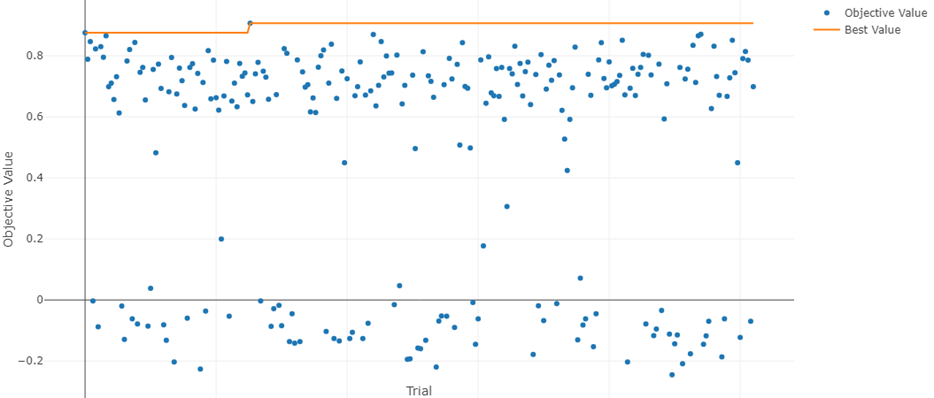
\includegraphics[width=15cm]{figures/figure-4.4.2.png}
% 	\caption[Trials Performance Distribution of RandomSampler - Experiment 4]{Scatter plot of the distribution of the performance of the trials of the RandomSampler in Experiment 4.}
% 	\label{fig:figure-4.4.2}
% \end{figure}
% 
% \begin{figure}[t]
% 	\centering
% 	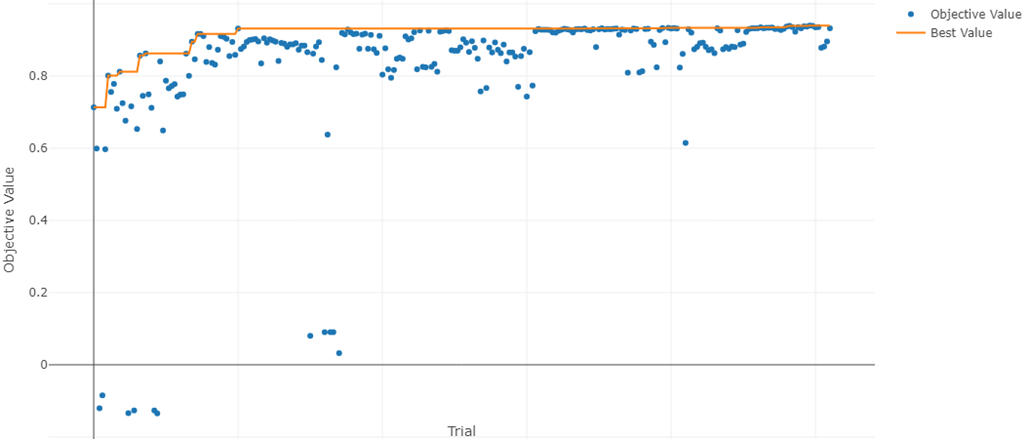
\includegraphics[width=15cm]{figures/figure-4.4.3.png}
% 	\caption[Trials Performance Distribution of TPESampler - Experiment 4]{Scatter plot of the distribution of the performance of the trials of the TPESampler in Experiment 4.}
% 	\label{fig:figure-4.4.3}
% \end{figure}
% 
% \begin{figure}[t]
% 	\centering
% 	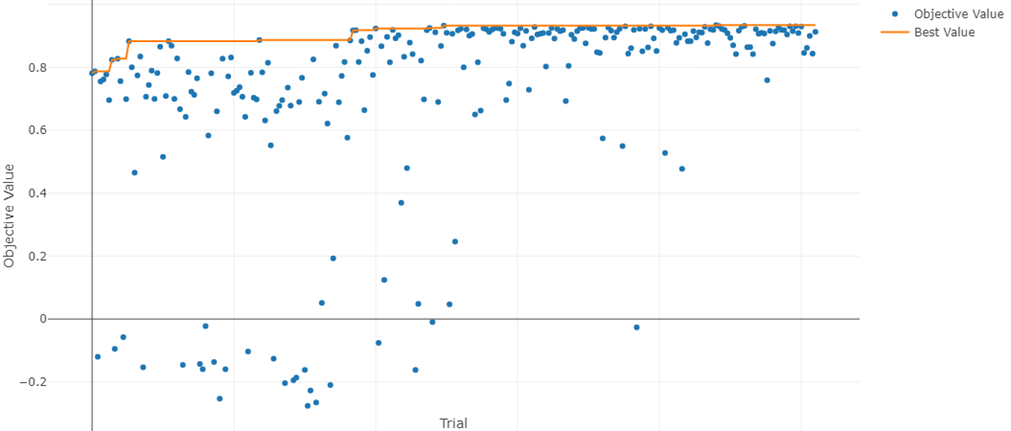
\includegraphics[width=15cm]{figures/figure-4.4.4.png}
% 	\caption[Trials Performance Distribution of PSOSampler - Experiment 4]{Scatter plot of the distribution of the performance of the trials of the PSOSampler in Experiment 4.}
% 	\label{fig:figure-4.4.4}
% \end{figure}
% 

\subsubsection{Analysis of the Hyperparameters Importance}

In this experiment, being all the sub-experiments part of Optuna, it was possible to use Optuna Storage to generate some plots.
\\[0.3cm]All three Samplers generated similar Hyperparameters Importance histograms. In all three, it is evident how the three hyperparameters associated with the layer width are not at the same level of importance, when they should be (Fig.~\ref{fig:figure-4.4.1}). The reason for this is not entirely clear, but it is probably again due to the fact that the problem is very simple, so almost any change in the hyperparameters can lead to a good result, moving away the focus from the importance of the architecture complexity.
\\[0.3cm]The most important hyperparameter appears to be the optimizer; this is probably as a result of the fact that there are only two optimizers, and Adam is almost always better than SGD, therefore making the final score obtain a great advantage.
\begin{figure}[H]
    \begin{minipage}{\textwidth}
        \centering
        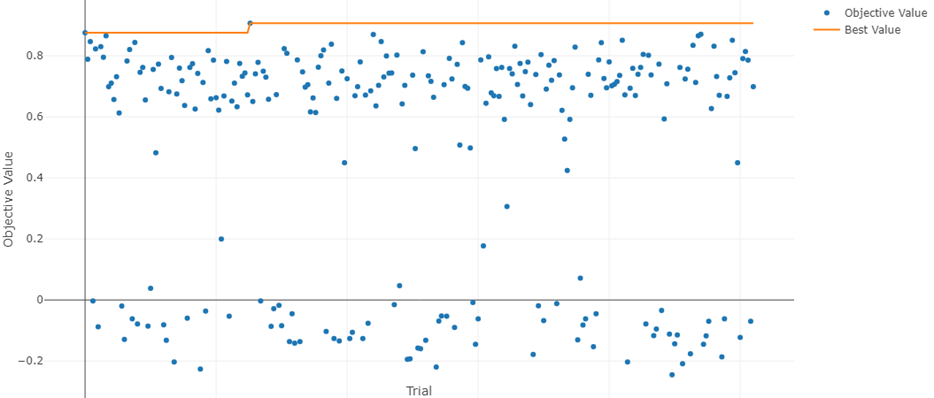
\includegraphics[width=13.8cm]{figures/figure-4.4.2.png}
        \caption[Trials Performance Distribution of RandomSampler - Experiment 4]{Scatter plot of the distribution of the performance of the trials of the RandomSampler in Experiment 4.}
        \label{fig:figure-4.4.2}
    \end{minipage}

    \begin{minipage}{\textwidth}
        \centering
        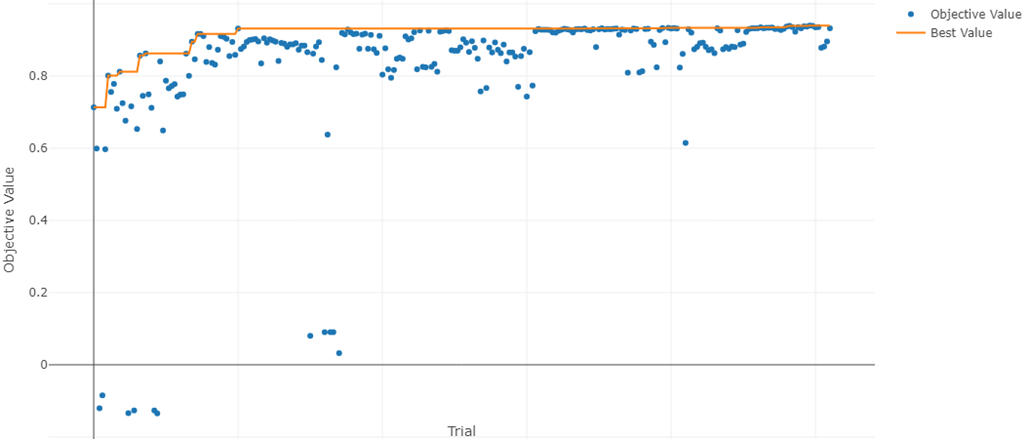
\includegraphics[width=13.8cm]{figures/figure-4.4.3.png}
        \caption[Trials Performance Distribution of TPESampler - Experiment 4]{Scatter plot of the distribution of the performance of the trials of the TPESampler in Experiment 4.}
        \label{fig:figure-4.4.3}
    \end{minipage}

    \begin{minipage}{\textwidth}
        \centering
        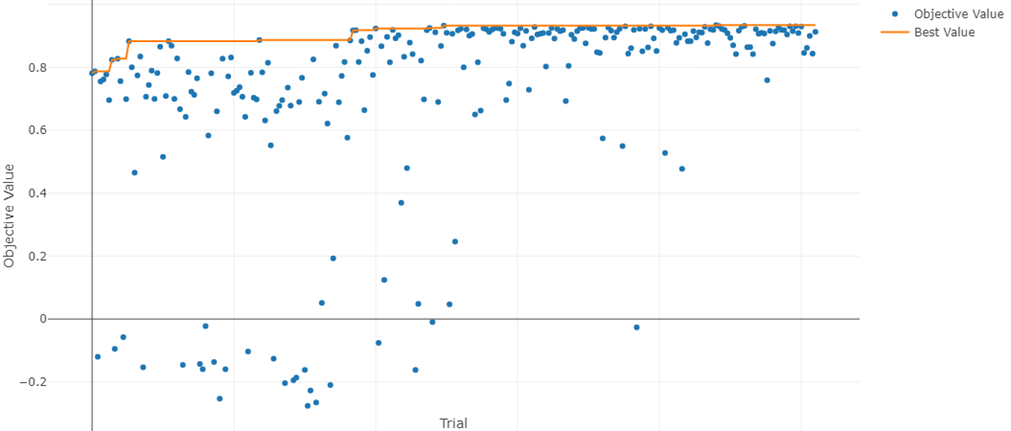
\includegraphics[width=13.8cm]{figures/figure-4.4.4.png}
        \caption[Trials Performance Distribution of PSOSampler - Experiment 4]{Scatter plot of the distribution of the performance of the trials of the PSOSampler in Experiment 4.}
        \label{fig:figure-4.4.4}
    \end{minipage}
\end{figure}
\begin{figure}[t]
	\centering
	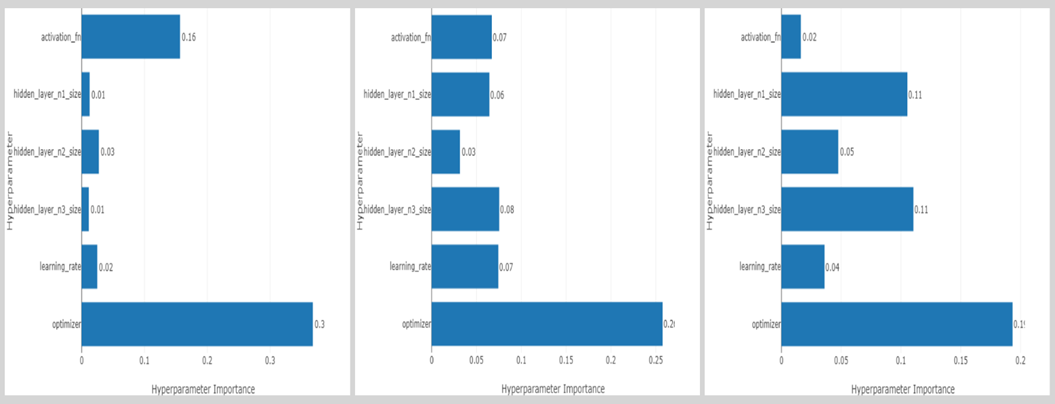
\includegraphics[width=15cm]{figures/figure-4.4.1.png}
	\caption[Hyperparameters Importance Histograms Experiment 4]{Comparison between the generated histograms of the importance of the hyperparameters of Experiment 4. From left to right, Studies of: RandomSampler, TPESampler, PSOSampler.}
	\label{fig:figure-4.4.1}
\end{figure}

\section[Experiment 5 - HPO on Weed Map Dataset]{Experiment 5 - Hyperparameter Optimization on Weed Map Dataset}

The goal of this experiment is to perform a Hyperparameter Optimization, using the samplers from the previous experiments, for a Weed Mapping problem.
\\[0.3cm]In Drone Vision, Semantic Segmentation is applied to identify immediately and automatically the different categories of “object” inside a cultivated field (crop, terrain, weed). But drones, especially those used for agriculture, do not carry powerful computers able to run complex Neural Networks Models.
\\[0.3cm]Therefore, it is necessary to execute a Hyperparameter Optimization of a NN model for Drone Vision, in order to find a candidate solution that is lightweight but does not lose too much generalization power.
\\[0.3cm]The model utilized for this experiment is Lawin, which is introduced in its relative section in the Methodology chapter (Sec.~\ref{sec:Lawin-3.4.1.2}).
\\[0.3cm]The Dataset of the experiment is Weed Map, a popular dataset for Drone Vision.

\myparagraph{System used for the Experiment:}
The hardware that was utilized to run this experiment is the following:
\begin{itemize}[itemsep=0.1cm]
	\item CPU: AMD EPYC 7V12(Rome) @ 2.45GHz (4-core)
	\item GPU: NVIDIA Tesla T4 (16GB VRAM)
	\item RAM: 28GB
	\item Disk: SSD
	\item OS: Linux (Ubuntu)
\end{itemize}
(This hardware is a Virtual Machine on the Azure ML servers).

\subsection{Weed Map Dataset}

\subsubsection{Introduction to Weed Map Dataset}

The Weed Map Dataset is the dataset for the research “WeedMap: A large-scale semantic weed mapping framework using aerial multispectral imaging and deep neural network for precision farming” \cite{Tesi-2.1}.
\\[0.3cm]Each picture of the Dataset shows an image of a cultivated field, where there can be distinguished Dirt, Weeds and Crops.
\\[0.3cm]The image below (Fig.~\ref{fig:figure-4.5.1}) is an example of one of the images. It is first shown the entire Orthomosaic Map, and then different zoom levels. This highlights the large scale of the image and the difficulty in distinguishing between Crops and Weeds.
\begin{figure}[t]
	\centering
	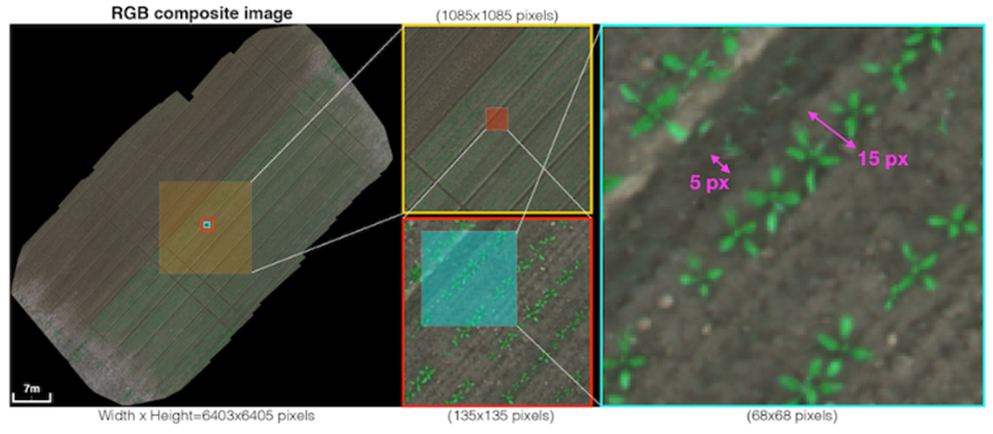
\includegraphics[width=14cm]{figures/figure-4.5.1.png}
	\caption[Example of image in Weed Map Dataset]{Example of image in Weed Map Dataset; with different zoom levels. Source:~\cite{Tesi-2.1}}
	\label{fig:figure-4.5.1}
\end{figure}

\myparagraph{Data Collection:}
The data included in the dataset was collected from aerial images (with Drones) from two different Sugar Beet fields: Eschikon (Switzerland) and Rheinbach (Germany). (Fig.~\ref{fig:figure-4.5.2})
\\[0.3cm]In particular, the utilized Drones are two commercial quadrotor UAVs, equipped with multispectral cameras.
\begin{figure}[t]
	\centering
	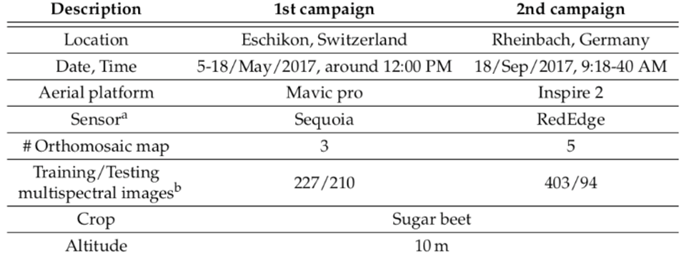
\includegraphics[width=13cm]{figures/figure-4.5.2.png}
	\caption[Information on Campaigns of Weed Map Dataset]{Information on the campaigns of data collection of Weed Map Dataset. Source:~\cite{Tesi-2.1}}
	\label{fig:figure-4.5.2}
\end{figure}

\subsubsection{Structure of Weed Map Dataset}

The full Dataset consist of 129 directories, for a total of 18746 image files. The total weight is 5.36GB.

\myparagraph{Folder Structure:}
There are two main folders, which are Orthomosaic and Tiles.
Orthomosaic contains the full orthomosaic maps.
Tiles contains, for each orthomosaic map, a folder containing images that represent cropped sections of the original orthomosaic map. All cropped sections together form the full map.
\\[0.3cm]Both Orthomosaic and Tiles contain RedEdge and Sequoia subfolders, containing 8 Orthomosaic maps in total (5 RedEdge and 3 Sequoia). (Fig.~\ref{fig:figure-4.5.3})
\\[0.3cm]Each Orthomosaic map stands in a folder indexed from 000 to 007.
\begin{figure}[t]
	\centering
	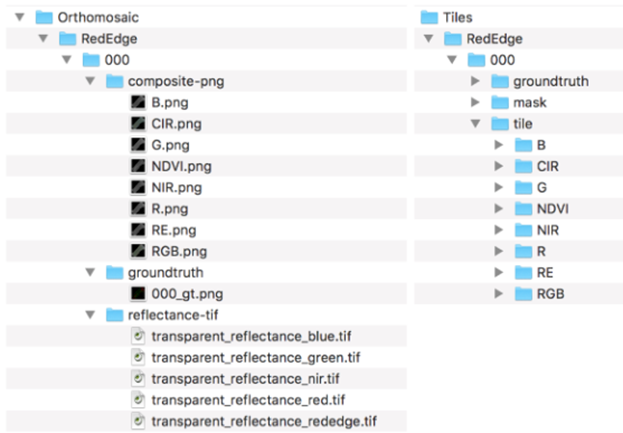
\includegraphics[width=10cm]{figures/figure-4.5.3.png}
	\caption[Folder Structure Weed Map Dataset]{Table showing the folder structure of Weed Map Dataset. Source:~\cite{Tesi-2.1}}
	\label{fig:figure-4.5.3}
\end{figure}

\myparagraph{Groundtruth:}
The Groundtruth images are pictures of the fields where each pixel has been manually labeled. (Fig.~\ref{fig:figure-4.5.4})
Each class is represented in a different colour:
\begin{itemize}[itemsep=0.1cm]
	\item Background (Dirt and part and part of the image which is not the crop field): is Black (code 0)
	\item Crops: is Green (code 1)
	\item Weeds: is Red (code 2)
\end{itemize}
The Groundtruth images are utilized to evaluate the precision of each prediction.
\begin{figure}[t]
	\centering
	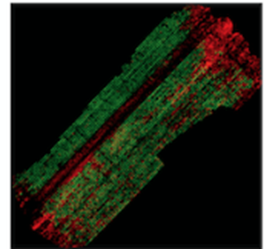
\includegraphics[width=5cm]{figures/figure-4.5.4.png}
	\caption[Example of GroundTruth in Weed Map Dataset]{Example of GroundTruth image in Weed Map Dataset. Source:~\cite{Tesi-2.1}}
	\label{fig:figure-4.5.4}
\end{figure}

\subsection{Preparation of the Experiment}

This experiment is partially different from the previous experiments. All studies continue to be initialized with the “wrapping”.
\\[0.3cm]The architectures with which to initialize the NN are no longer built inside the objective function, and thus need to be defined earlier. The architectures subject of this experiment are defined in the same article in which the original experiment of Weed Mapping was proposed \cite{WeedMap-PaperThesis}. During the experiment, those architectures will be referenced as “backbone”.
\\[0.3cm]The Weed Map dataset was loaded using the pre-defined function mentioned in the related section of the Methodology chapter (Sec.~\ref{sec:Lawin-3.4.1.2}). The utilized version of Weed Map Dataset is not the original version, but is a pre-processed one (the same as \cite{WeedMap-PaperThesis}).

\subsubsection{Setup of the Studies}

% \myparagraph{Initialize the Studies:}
The samplers of Optuna used to perform three different HPOs, are the following: \texttt{RandomSampler}, \texttt{TPESampler}, \texttt{PSOSampler}.
For each of the samplers, an Optuna \texttt{Study} is created. All the standard samplers are initialized with their default input values. The \texttt{PSOSampler} is initialized with two values, \texttt{num\_particles} and \texttt{max\_generations}.
\\[0.3cm]The Pruning mechanism used is the Median Pruning algorithm. It is applied through the \texttt{MedianPruner} object of Optuna, whose values for initialization are below.

\subsubsection{Setup of the Objective Function}

% \myparagraph{Objective Function:}
The objective function, as always, is the same for each Study. The structure of the objective function is the same as in the last experiments.
\\[0.3cm]It is important to note one difference, which is the metric to follow. Although all four metrics are always computed, in this experiment the F1-Score will be the main metric, differently from the previous experiments where it was Accuracy.
\\[0.3cm]The initialization hyperparameters of the loss function, \texttt{Focal}, were fixed. Their chosen values are: \texttt{gamma} = 2, \texttt{weights} = [0.06, 1, 1.7].
% 
% \myparagraph{Search Space of Hyperparameters:}
\\[0.3cm]The Hyperparameters declared in the objective function, which form the Search Space of the Study, for this experiment were the following (Tab.~\ref{tab:table-4.5.1}).
\begin{table}[ht!]
	\center
	\setlength{\tabcolsep}{0.5cm}
	\caption[Search Space of Experiment 5]{Search Space of Experiment 5: list of hyperparameters and their values ranges, with the step. Where Step is $\sim$ if the range is continuous.}
	\begin{tabular}{@{}lcc@{}}
		\toprule
		\textbf{Hyperparamter} & \textbf{Range}                             & \textbf{Step} \\ \midrule
		Backbone               & \{MiT-B0, MiT-LD, MiT-L0, MiT-L1, MiT-L2\} & -             \\[0.1cm]
		Learning Rate          & {[}$10^{-4}$, $10^{-2}${]}                 & $\sim$        \\[0.1cm]
		Optimizer              & \{SGD, Adam\}                              & -             \\ \bottomrule
	\end{tabular}
	\label{tab:table-4.5.1}
\end{table}
% 
% \myparagraph{Optimizing Process Parameters:}
\\[0.3cm]Other parameters, related to the Optimization process, basically hyperparameters of the HPO process itself (could be called “Hyper-Hyperparamters”), which were used are the following (Tab.~\ref{tab:table-4.5.2}).
\begin{table}[ht!]
	\center
	\setlength{\tabcolsep}{0.5cm}
	\caption[Optimization External Parameters of Experiment 5]{External optimization parameters of Experiment 5, basically hyperparameters of the optimization process, with their values.}
	\begin{tabular}{@{}llc@{}}
		\toprule
		\textbf{Group}                & \textbf{Parameter} & \textbf{Value} \\ \midrule
		Regularizer                   & labda              & 0.4            \\[0.1cm]
		EarlyStopper                  & patience           & 15             \\[0.2cm]
		\multirow{2}{*}{PSOSampler}   & num\_particles     & 32             \\[0.1cm]
									  & max\_generations   & 8              \\[0.2cm]
		\multirow{4}{*}{MedianPruner} & n\_startup\_trials & 2              \\[0.1cm]
									  & n\_warmup\_steps   & 20             \\[0.1cm]
									  & interval\_steps    & 20             \\[0.1cm]
									  & n\_min\_trials     & 4              \\ \bottomrule
	\end{tabular}
	\label{tab:table-4.5.2}
\end{table}

\subsection{Execution of the Experiment}

The execution of each Study is handled by an OptunaRunner object for Optuna, which at the end of the optimization process saves the results on a csv file.
\\[0.3cm]The number of Trials executed for each Study was 64.

\subsubsection{Score Results}

The best score achieved by the \texttt{RandomSampler} is 70\%; the top trials have as backbone MiT-L1 and MiT-L2; F1-Score of the best trials is around 69\%-74\%.
\\[0.3cm]The best score achieved by the \texttt{TPESampler} is 74.4\%; the top trials have as backbone MiT-L2; the F1-Score of the best trials is around 70\%-77\%.
\\[0.3cm]The best score achieved by the \texttt{PSOSampler} is 70.1\%; the top trials have as backbone MiT-L2 (the best one MiT-L1); the F1-Score of the best trials is around 70\%-75\%.
\\[0.3cm]For all three samplers, the best trials in terms of F1-Score have as backbones MiT-B0 and MiT-LD.

\subsubsection{Hyperparameters Results}

The Hyperparameters Importance graph is shown in the figure (Fig.~\ref{fig:figure-4.5.5}), which is the one generated from \texttt{TPESampler}, being the Study with the best results, even though also the other two studies generated very similar results.
\begin{figure}[t]
	\centering
	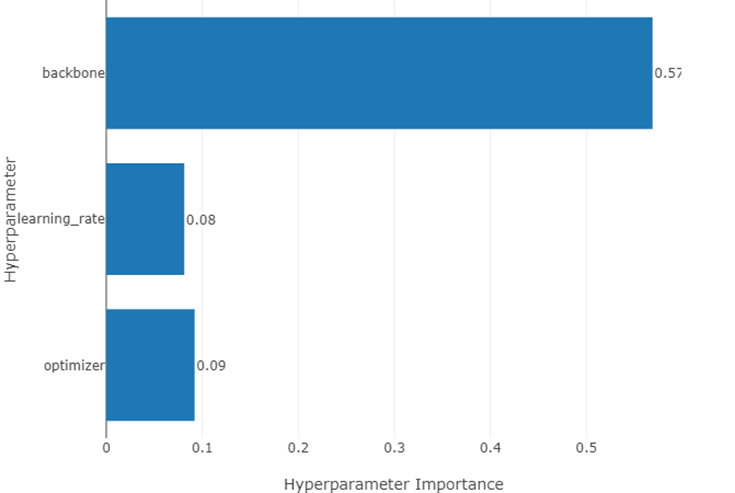
\includegraphics[width=13cm]{figures/figure-4.5.5.png}
	\caption[Hyperparameters Importance Histogram Experiment 5]{Histogram of the importance of the hyperparameters of Experiment 5, generated by the Study of TPESampler.}
	\label{fig:figure-4.5.5}
\end{figure}
\\[0.3cm]The best candidate solution, and thus the best found hyperparameters are:
\begin{itemize}[itemsep=0.1cm]
    \item Backbone = MiT-L2
    \item Learning Rate = 0.002
    \item Optimizer = Adam
\end{itemize}

\subsection{Discussion of the Results}

The results the of experiment allowed to find a valid hyperparameters' configuration that solves the initial problem.
In fact, the proposed solution, uses the most lightweight among all the Backbones, creating the most lightweight Neural Network for the Drone Vision problem possible.

\subsubsection{Analysis of the Performance of the Samplers}

The \texttt{RandomSampler} worked as usual, there does not seem to be any problem with its functioning. The \texttt{TPESampler} found good solutions, therefore, it could be argued that it is working as supposed. The \texttt{PSOSampler} on the other hand, showed results slightly below expectations.
\\[0.3cm]The reason \texttt{PSOSampler} underperformed in this particular experiment, is because of the way pruning influences the sampler in more complex problems like this experiment.
Differently from \texttt{TPESampler}, where there is only a “global perspective”, \texttt{PSOSampler} suffers a significantly more from pruning.
This is because the PSO algorithm is based on the concept of particles that move in a space, and the pruning mechanism removes some of the information that the particles need to move correctly.
Specifically, the trials of the particles that are not near the global optimum are pruned most of the time, not allowing the particles to update their Local Optimum. Thus, the Cognitive Factor of those particles becomes basically useless, and only the Social Factor matters. This causes a slowdown in the convergence of the algorithm, leading to worse results compared to other samplers like \texttt{TPESampler}.
\\[0.3cm]Potential fixes for this problem could be to remove the pruning mechanism for the \texttt{PSOSampler} (but this would make the process very computationally expensive), or to modify the pruning mechanism to be less aggressive, to allow the worst-positioned particles to continue to explore the space.  

\subsubsection{Analysis of the Quality of Results}

The considered results for this analysis are the ones from the \texttt{TPESampler}, as it was the sub-experiment with the best results among all samplers.
\\[0.3cm]The best solutions all have in common the same Backbone, which is MiT-L2. This is the lightest Backbone among the proposed ones.
Tested singularly with already known good hyperparameters, the MiT-B0 and MiT-LD, which are deeper, more complex architectures, have obtained results around 76\% of F1-Score on the Test Set.
The best solution obtained by the \texttt{TPESampler} with the MiT-L2 architecture obtained a F1-Score of 74.4\%, which is only 1.6\% apart from the best architecture.
\\[0.3cm]Therefore, this experiment could be considered a success, as the architecture of the Neural Network was heavily simplified from a total of 1024 neurons to 64 (MiT-B0 and MiT-L2 respectively), losing only 1.6\% from the performance.





%\chapter{Discussion}

\lipsum  % Replace with your text

\chapter{Conclusions}

The summary, as the last section of the text, includes clear and critical statements about:
\begin{itemize}
  \item The results of the work and their importance;
  \item The limits of validity and the progress compared with the level of knowledge at the beginning of the work;
  \item The applicability of the results; and, possibly
  \item Recommendations for further tasks.
\end{itemize}

% -------------------------------------------------------------------
% Bibliography
% -------------------------------------------------------------------

\bibliographystyle{unsrtnat}
\bibliography{main} 

% -------------------------------------------------------------------
% Appendices
% -------------------------------------------------------------------

%\begin{appendices}
%\chapter{An Appendix of Some Kind}

\lipsum[1-3]  % Replace with your text

%\chapter{Another Appendix}

\lipsum[1-3]  % Replace with your text

%\end{appendices}

\end{document}
